
% AGUJournalTemplate.tex: this template file is for articles formatted with LaTeX
%
% This file includes commands and instructions
% given in the order necessary to produce a final output that will
% satisfy AGU requirements, including customized APA reference formatting.
%
% You may copy this file and give it your
% article name, and enter your text.
%
%
% Step 1: Set the \documentclass
%
%

%% To submit your paper:
\documentclass[draft]{agujournal2019}
\usepackage{url} %this package should fix any errors with URLs in refs.
\usepackage{lineno}
\usepackage[inline]{trackchanges} %for better track changes. finalnew option will compile document with changes incorporated.
\usepackage{soul}
\linenumbers

%%%%%%%
% As of 2018 we recommend use of the TrackChanges package to mark revisions.
% The trackchanges package adds five new LaTeX commands:
%
%  \note[editor]{The note}
%  \annote[editor]{Text to annotate}{The note}
%  \add[editor]{Text to add}
%  \remove[editor]{Text to remove}
%  \change[editor]{Text to remove}{Text to add}
%
% complete documentation is here: http://trackchanges.sourceforge.net/
%%%%%%%

\draftfalse

%% Enter journal name below.
%% Choose from this list of Journals:
%
% JGR: Atmospheres
% JGR: Biogeosciences
% JGR: Earth Surface
% JGR: Oceans
% JGR: Planets
% JGR: Solid Earth
% JGR: Space Physics
% Global Biogeochemical Cycles
% Geophysical Research Letters
% Paleoceanography and Paleoclimatology
% Radio Science
% Reviews of Geophysics
% Tectonics
% Space Weather
% Water Resources Research
% Geochemistry, Geophysics, Geosystems
% Journal of Advances in Modeling Earth Systems (JAMES)
% Earth's Future
% Earth and Space Science
% Geohealth
%
% ie, \journalname{Water Resources Research}

\journalname{Journal of Advances in Modeling Earth Systems (JAMES)}


\begin{document}

%% ------------------------------------------------------------------------ %%
%  Title
%
% (A title should be specific, informative, and brief. Use
% abbreviations only if they are defined in the abstract. Titles that
% start with general keywords then specific terms are optimized in
% searches)
%
%% ------------------------------------------------------------------------ %%

% Example: \title{This is a test title}

\title{Impact of grids and dynamical cores in CESM2.2 on the meteorology and climate of the Arctic}

%% ------------------------------------------------------------------------ %%
%
%  AUTHORS AND AFFILIATIONS
%
%% ------------------------------------------------------------------------ %%

% Authors are individuals who have significantly contributed to the
% research and preparation of the article. Group authors are allowed, if
% each author in the group is separately identified in an appendix.)

% List authors by first name or initial followed by last name and
% separated by commas. Use \affil{} to number affiliations, and
% \thanks{} for author notes.
% Additional author notes should be indicated with \thanks{} (for
% example, for current addresses).

% Example: \authors{A. B. Author\affil{1}\thanks{Current address, Antartica}, B. C. Author\affil{2,3}, and D. E.
% Author\affil{3,4}\thanks{Also funded by Monsanto.}}
\authors{Adam R. Herrington \affil{1}, Marcus Lofverstrom \affil{2}, Peter H. Lauritzen \affil{1} and Andrew Gettelman \affil{1}}

 \affiliation{1}{National Center for Atmospheric Research, 1850 Table Mesa Drive, Boulder, Colorado, USA}
\affiliation{2}{Department of Geosciences, University of Arizona, 1040 E. 4th Street, Tucson, AZ USA}

% \affiliation{1}{First Affiliation}
% \affiliation{2}{Second Affiliation}
% \affiliation{3}{Third Affiliation}
% \affiliation{4}{Fourth Affiliation}

%\affiliation{=number=}{=Affiliation Address=}
%(repeat as many times as is necessary)

%% Corresponding Author:
% Corresponding author mailing address and e-mail address:

% (include name and email addresses of the corresponding author.  More
% than one corresponding author is allowed in this LaTeX file and for
% publication; but only one corresponding author is allowed in our
% editorial system.)

% Example: \correspondingauthor{First and Last Name}{email@address.edu}

\correspondingauthor{=name=}{=email address=}

%% Keypoints, final entry on title page.

%  List up to three key points (at least one is required)
%  Key Points summarize the main points and conclusions of the article
%  Each must be 140 characters or fewer with no special characters or punctuation and must be complete sentences

% Example:
% \begin{keypoints}
% \item	List up to three key points (at least one is required)
% \item	Key Points summarize the main points and conclusions of the article
% \item	Each must be 140 characters or fewer with no special characters or punctuation and must be complete sentences
% \end{keypoints}

\begin{keypoints}
\item enter point 1 here
\item enter point 2 here
\item enter point 3 here
\end{keypoints}

%% ------------------------------------------------------------------------ %%
%
%  ABSTRACT and PLAIN LANGUAGE SUMMARY
%
% A good Abstract will begin with a short description of the problem
% being addressed, briefly describe the new data or analyses, then
% briefly states the main conclusion(s) and how they are supported and
% uncertainties.

% The Plain Language Summary should be written for a broad audience,
% including journalists and the science-interested public, that will not have 
% a background in your field.
%
% A Plain Language Summary is required in GRL, JGR: Planets, JGR: Biogeosciences,
% JGR: Oceans, G-Cubed, Reviews of Geophysics, and JAMES.
% see http://sharingscience.agu.org/creating-plain-language-summary/)
%
%% ------------------------------------------------------------------------ %%

%% \begin{abstract} starts the second page

\begin{abstract}
[ enter your Abstract here ]
\end{abstract}

\section*{Plain Language Summary}
[ enter your Plain Language Summary here or delete this section]


%% ------------------------------------------------------------------------ %%
%
%  TEXT
%
%% ------------------------------------------------------------------------ %%

%%% Suggested section heads:
\section{Introduction}

General Circulation Models (GCMs) are powerful tools for understanding the meteorology and climate of the high-latitudes, which are among the most sensitive regions on Earth to global and environmental change. Despite their importance, the numerical treatment of polar regions is handled in vastly-different ways due to the so-called \textit{pole-problem} \cite{W2007JMSJ}. The pole-problem refers to instability arising from the convergence of meridians at the polar points on latitude-longitude grids (e.g., Figure~\ref{fig:uni-grids}a). Depending on the numerics, methods exist to stabilize the pole problem, and latitude-longitude grids may be advantageous for polar processes as structures can be represented with more degrees of freedom than elsewhere in the computational domain. With the recent trend towards globally uniform unstructured grids, any potential benefits of latitude-longitude grids on polar regions may become a relic of the past. In this study, a spectrum of grids and dynamical cores (hereafter referred to as \textit{dycores}) available in the Community Earth System Model, version 2.2 (CESM; \url{http://www.cesm.ucar.edu/models/cesm2/}), from conventional latitude-longitude grids to unstructured grids with globally uniform grid spacing to unstructured grids with regional refinement over the Arctic, are evaluated to understand their impacts on the simulated characteristics of the Arctic, with a special focus on the Greenland Ice Sheet.

In the 1970's the pole problem was largely defeated through wide-spread adoption of efficient spectral transform methods in GCMs. These methods transform grid point fields into a global, isotropic representation in wave space, where linear operators in the equation set can be solved for exactly. While spectral transform methods are still commonly used in the 21st century, local numerical methods have become desirable for their ability to run efficiently on massively parallel systems. The pole-problem has thus re-emerged in contemporary climate models that use latitude-longitude grids, and some combination of reduced grids and polar filters are necessary to ameliorate this instability \cite{JW2010LNCSE}. Polar filters are akin to a band-aid; they subdue the growth of unstable modes by applying additional damping to the solution over polar regions. One might expect that this additional damping reduces the effective resolution such that the resolved scales are similar across the entire domain, but this seems an unlikely outcome and is explored further in this study.

An alternative approach is to use unstructured grids. Unstructured grids allow for more flexible grid structures, permitting quasi-uniform grid spacing globally that eliminates the pole-problem entirely (e.g., Figure~\ref{fig:uni-grids}c). This grid flexibility also allows for variable-resolution or regional grid refinement. Grids can be developed with refinement over polar regions that could in principle make up for any loss in polar resolution in transitioning away from latitude-longitude grids (e.g., Figure~\ref{fig:vr-grids}), although this comes at the cost of a smaller CFL-limiting time-step in the refined region. But unstructured grids scale more efficiently on parallel systems than latitude-longitude grids, resulting in latitude-longitude grids becoming less common, and unstructured grids more common as computing power continued to increase over time.

The meteorology and climate of the Arctic is characterized by a range of processes and scales that are difficult to represent in GCMs \cite{BETAL2001MWR,SG2017MWR,VETAL2018TC}. Synoptic scale storms are well represented at typical GCM resolutions, but mesoscale Polar Lows are not. These mesoscale systems are prevalent during the cold season, and produce gale-force winds that can induce large fluxes through the underlying sea-ice/ocean interface. The Arctic also contains the Greenland Ice Sheet (hereafter denoted as \textit{GrIS}). While it blankets the largest island in the world (Greenland), GrIS is only marginally resolved at typical GCM resolutions. GrIS ablation zones exert a primary control on the mass balance of the ice sheet, but are on the order of 100km wide, and models struggle to resolve these narrow features. GrIS elevations descends rapidly toward the coasts, resulting in steep margins that facilitate orographic precipitation events, but which are not well resolved in GCMs. The Arctic is therefore well-suited to understand the impact of different grids and dycores on processes that are marginally resolved at conventional GCM resolutions.

The goal of this study is to characterize the representation of high-latitude regions using the spectral-element and finite-volume dycores in CESM2.2, as these models treat the high-latitudes, e.g., the pole-problem, in very different ways. The manuscript is laid out as follows. Section~\ref{sec:methods} consists of documentation of the grids, dycores and physical parameterizations used in this study. The Arctic refined grids were developed by the authors, and this section serves as their official documentation in CESM2.2. Section~\ref{sec:methods} also contains a description of the experiments along with the observational datasets and post-processing software used for evaluating the models. Section~\ref{sec:results} contains the results of the experiments and Section~\ref{sec:conclusions} provides some discussion and conclusions. 

\begin{figure}[t]
\begin{center}
\begin{tabular}{cc}
         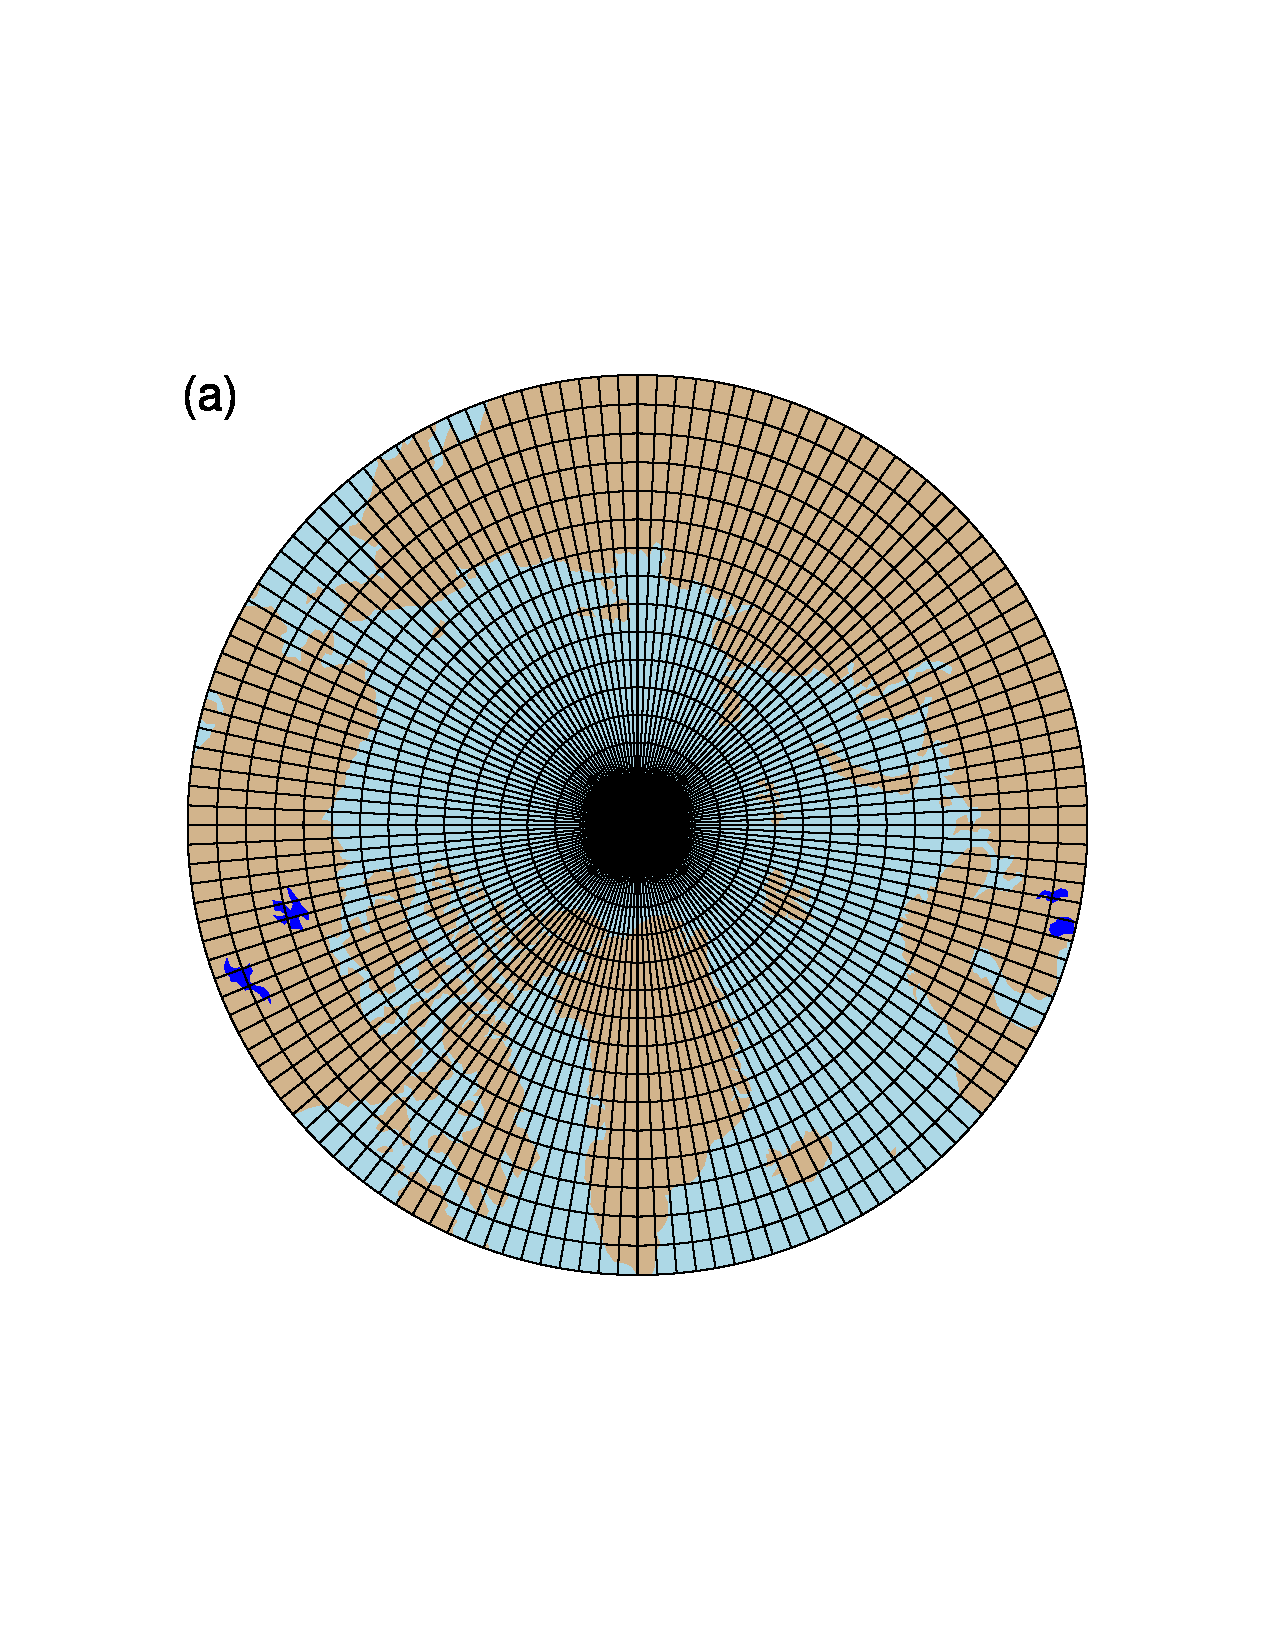
\includegraphics[width=60mm]{figs/grid-f19.pdf}&
         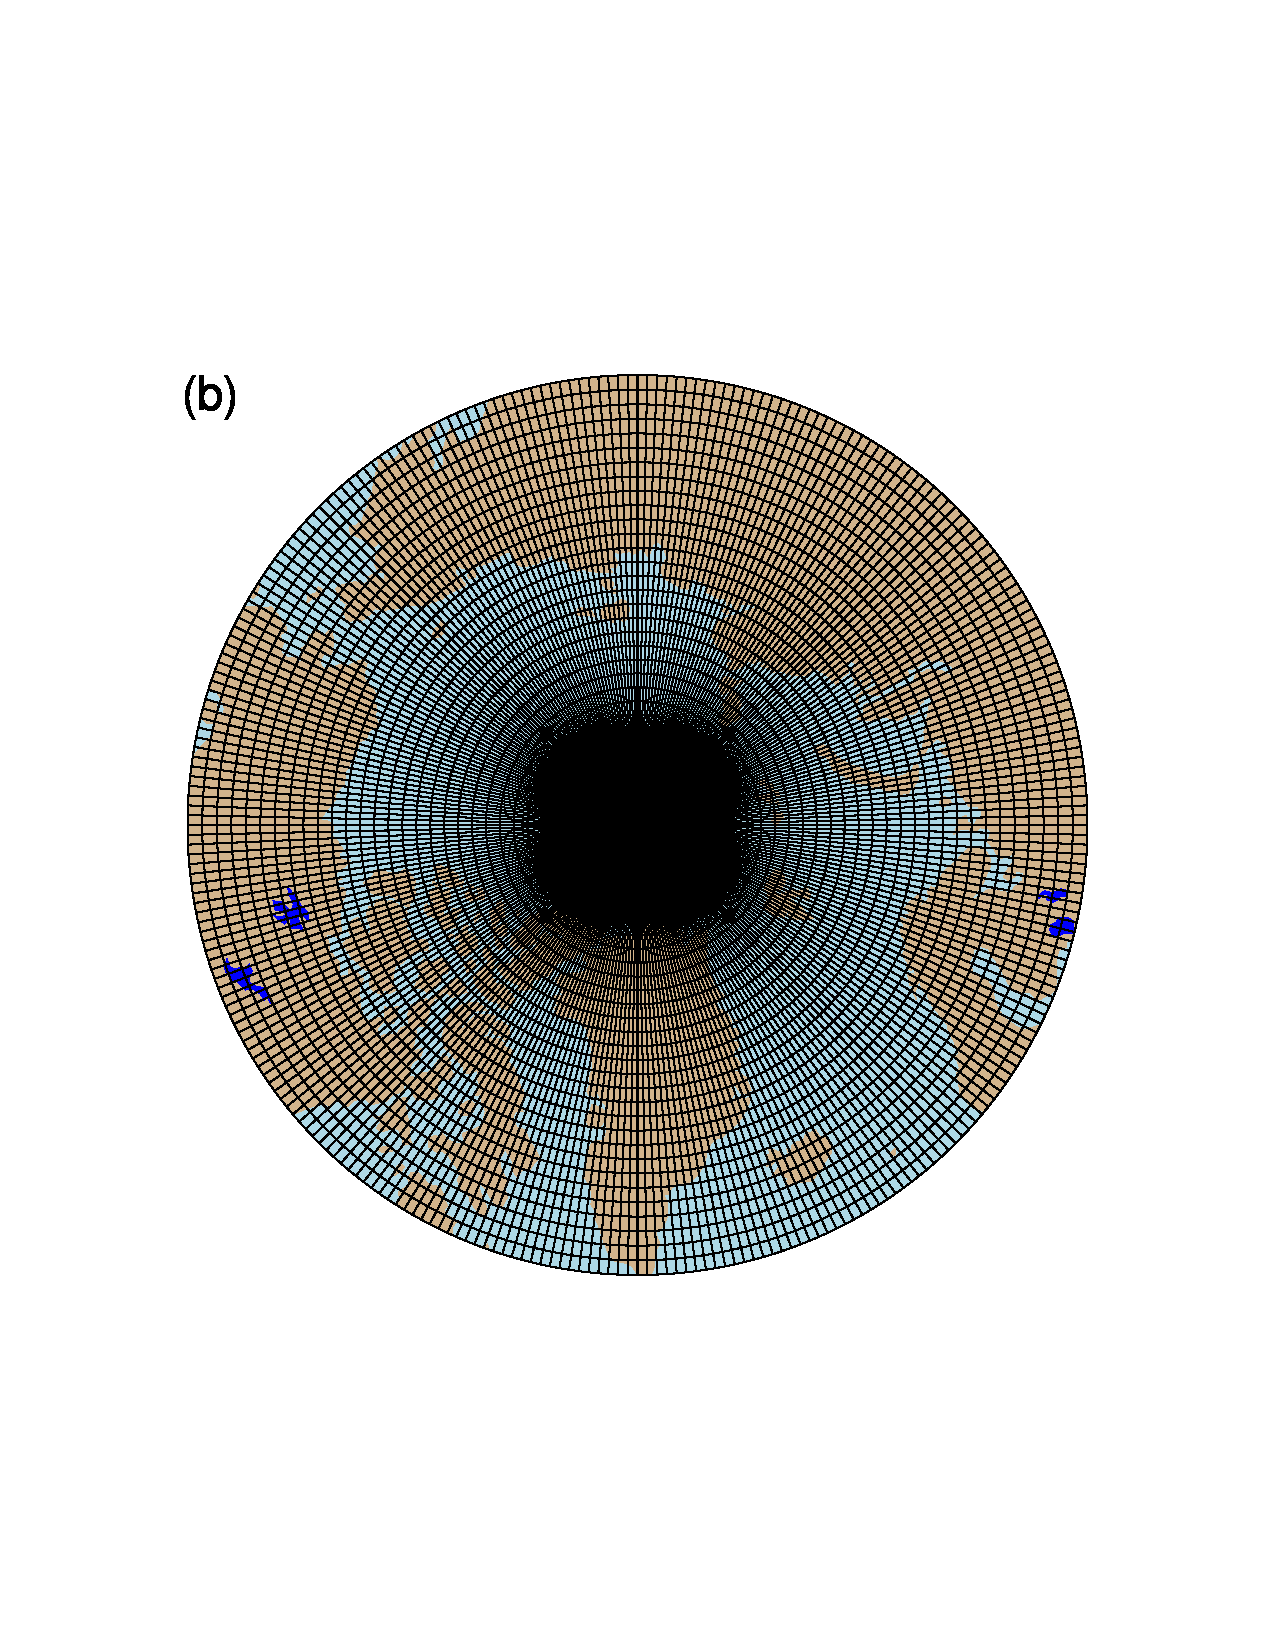
\includegraphics[width=60mm]{figs/grid-f09.pdf}\\
         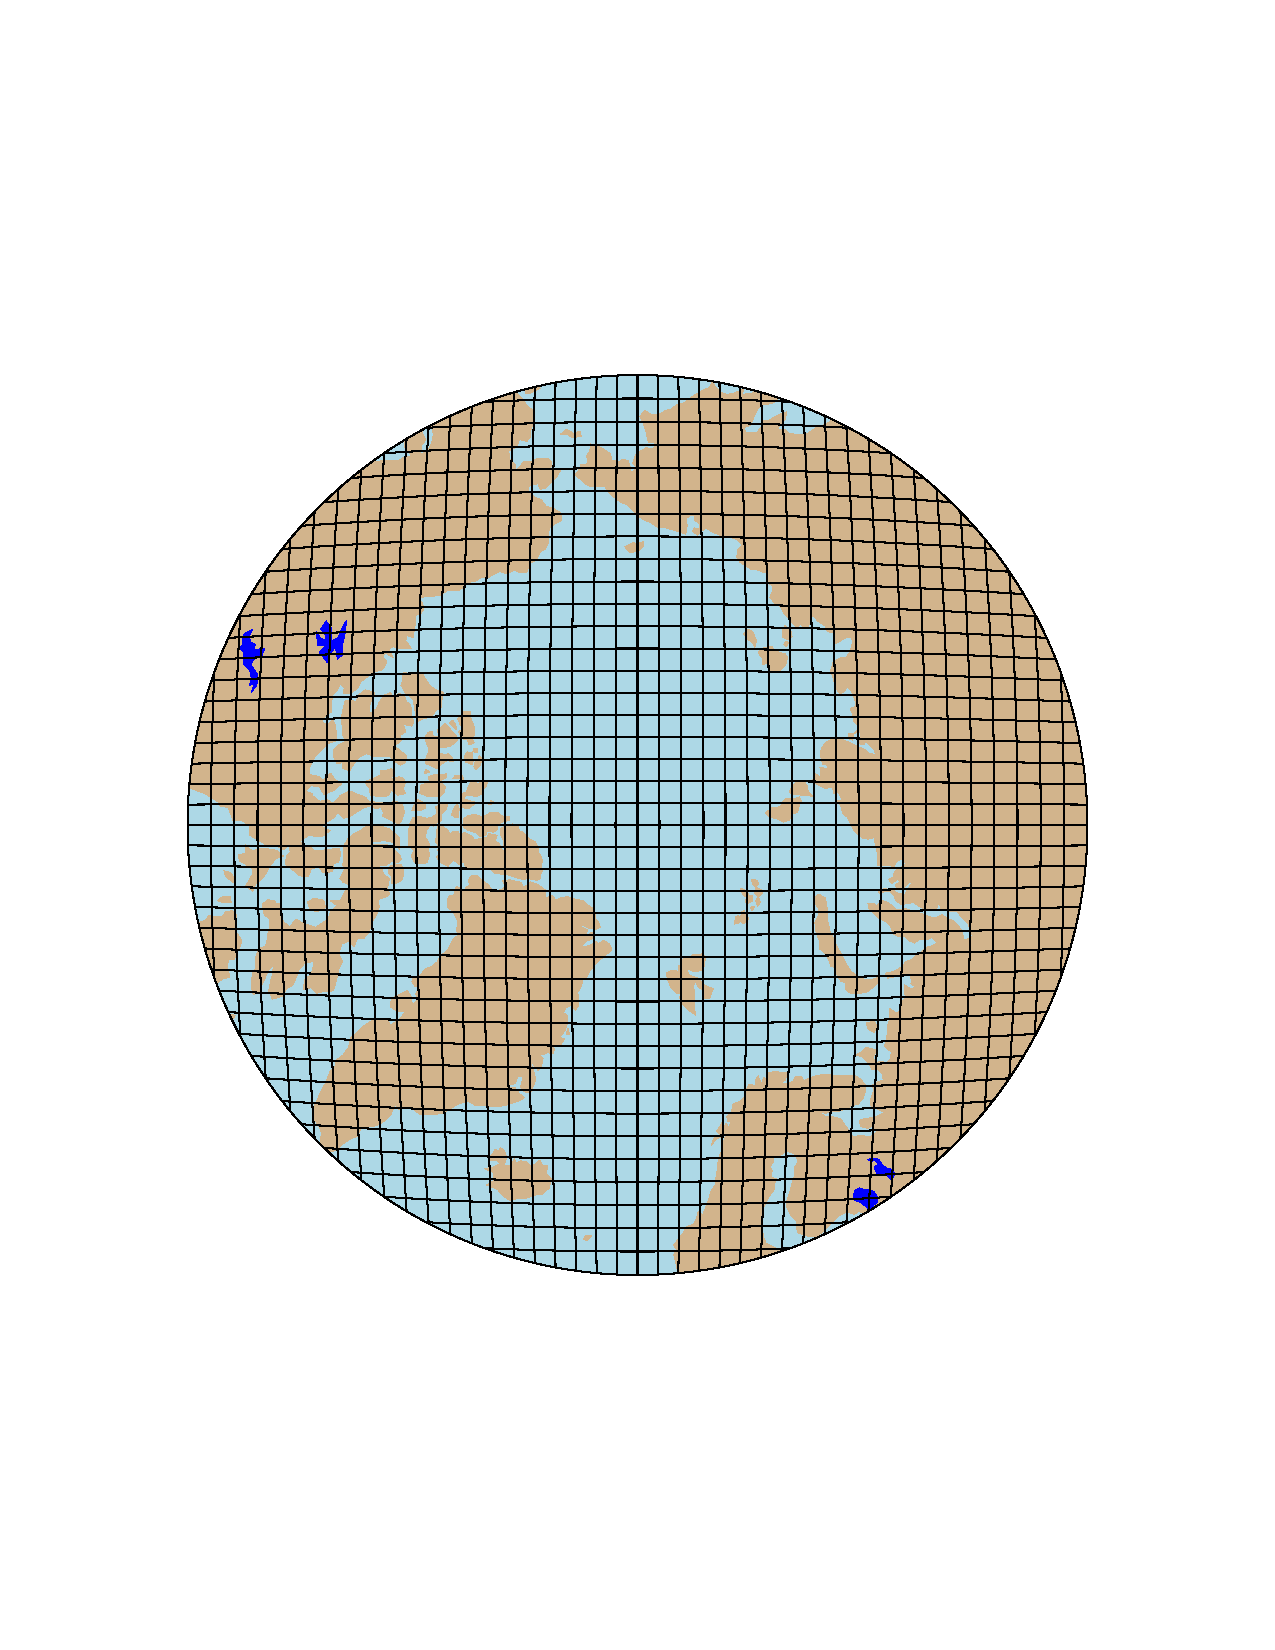
\includegraphics[width=60mm]{figs/grid-ne30pg2.pdf}&
         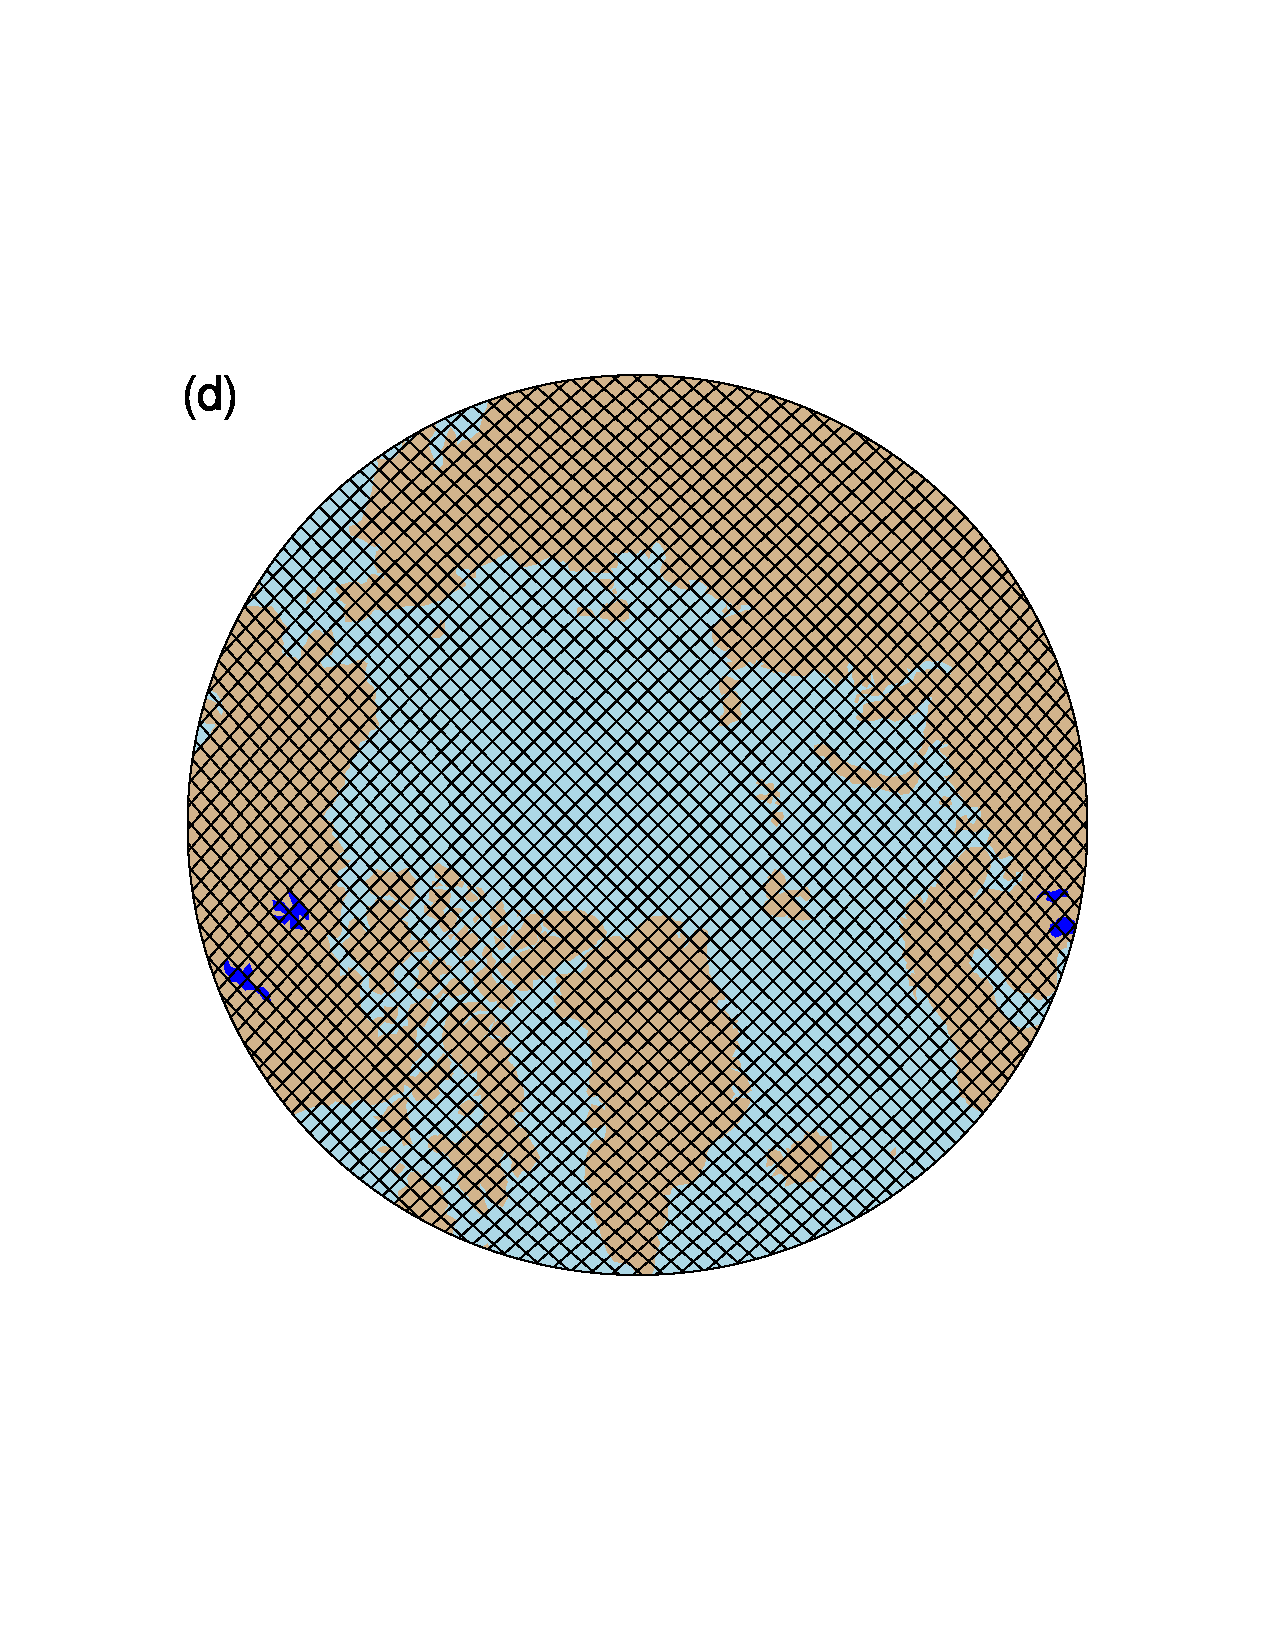
\includegraphics[width=60mm]{figs/grid-ne30pg3.pdf} \\
\end{tabular}
\end{center}
\caption{.}
\label{fig:uni-grids}
\end{figure}

\begin{figure}[t]
\begin{center}
\begin{tabular}{cccc}
         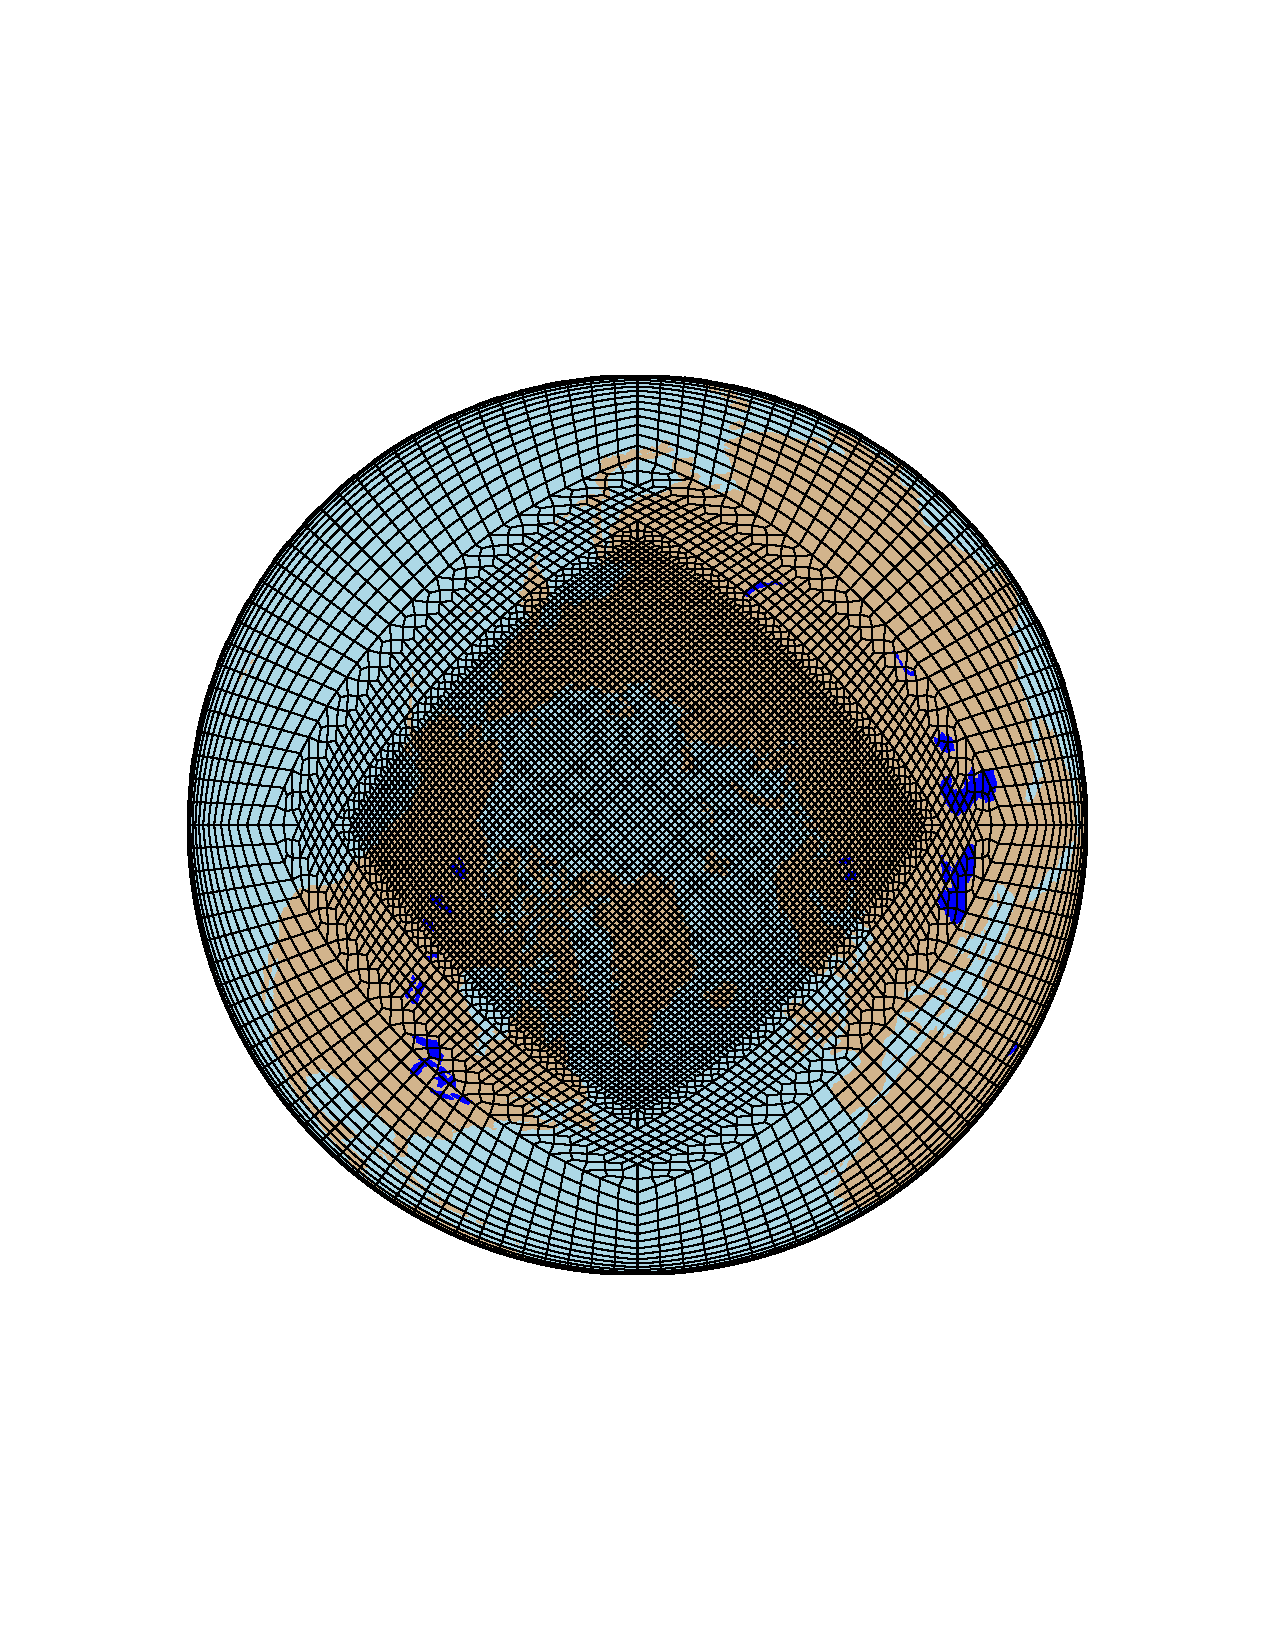
\includegraphics[width=60mm]{figs/grid-ARCTIC.pdf}&
         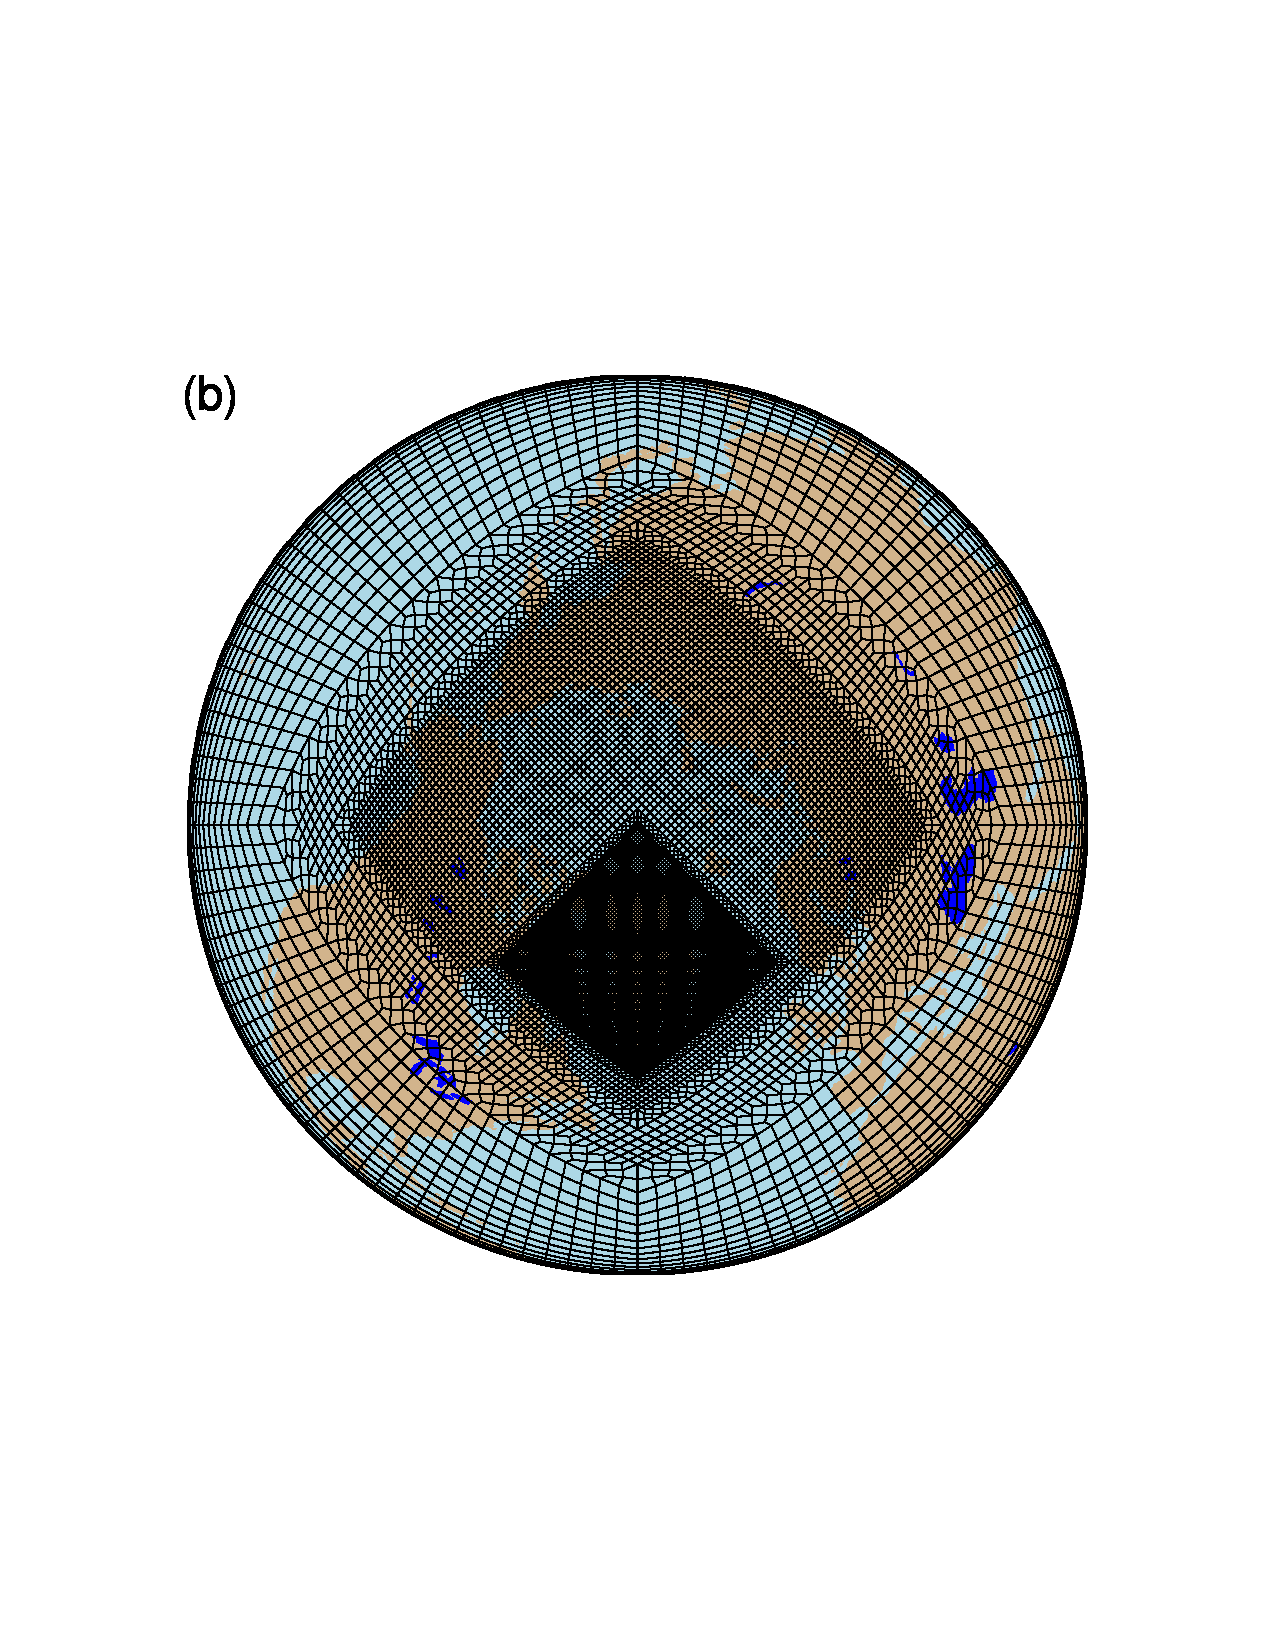
\includegraphics[width=60mm]{figs/grid-ARCTICGRIS.pdf} \\
\end{tabular}
\end{center}
\caption{.}
\label{fig:vr-grids}
\end{figure}

\begin{figure}[t]
\begin{center}
\begin{tabular}{cccc}
         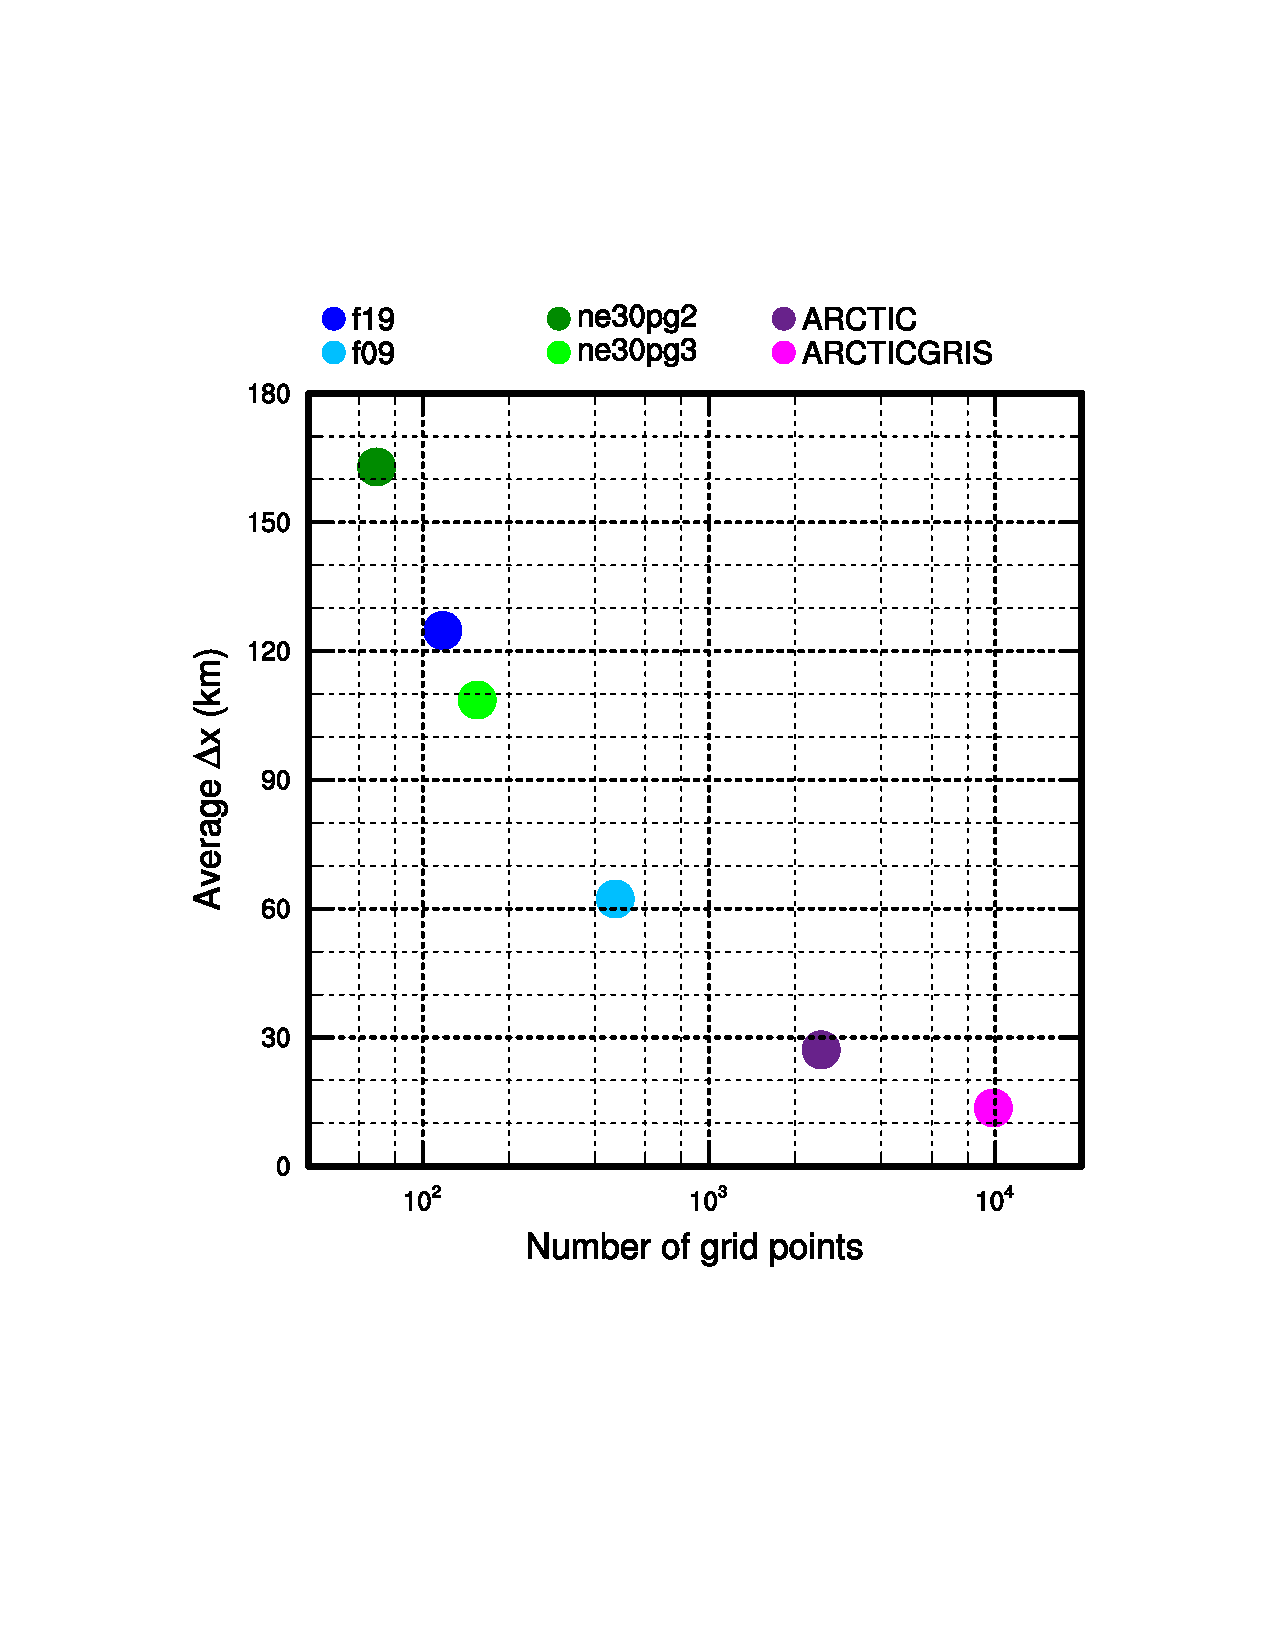
\includegraphics[width=60mm]{figs/temp_grisres_dxoverglc.pdf}&
         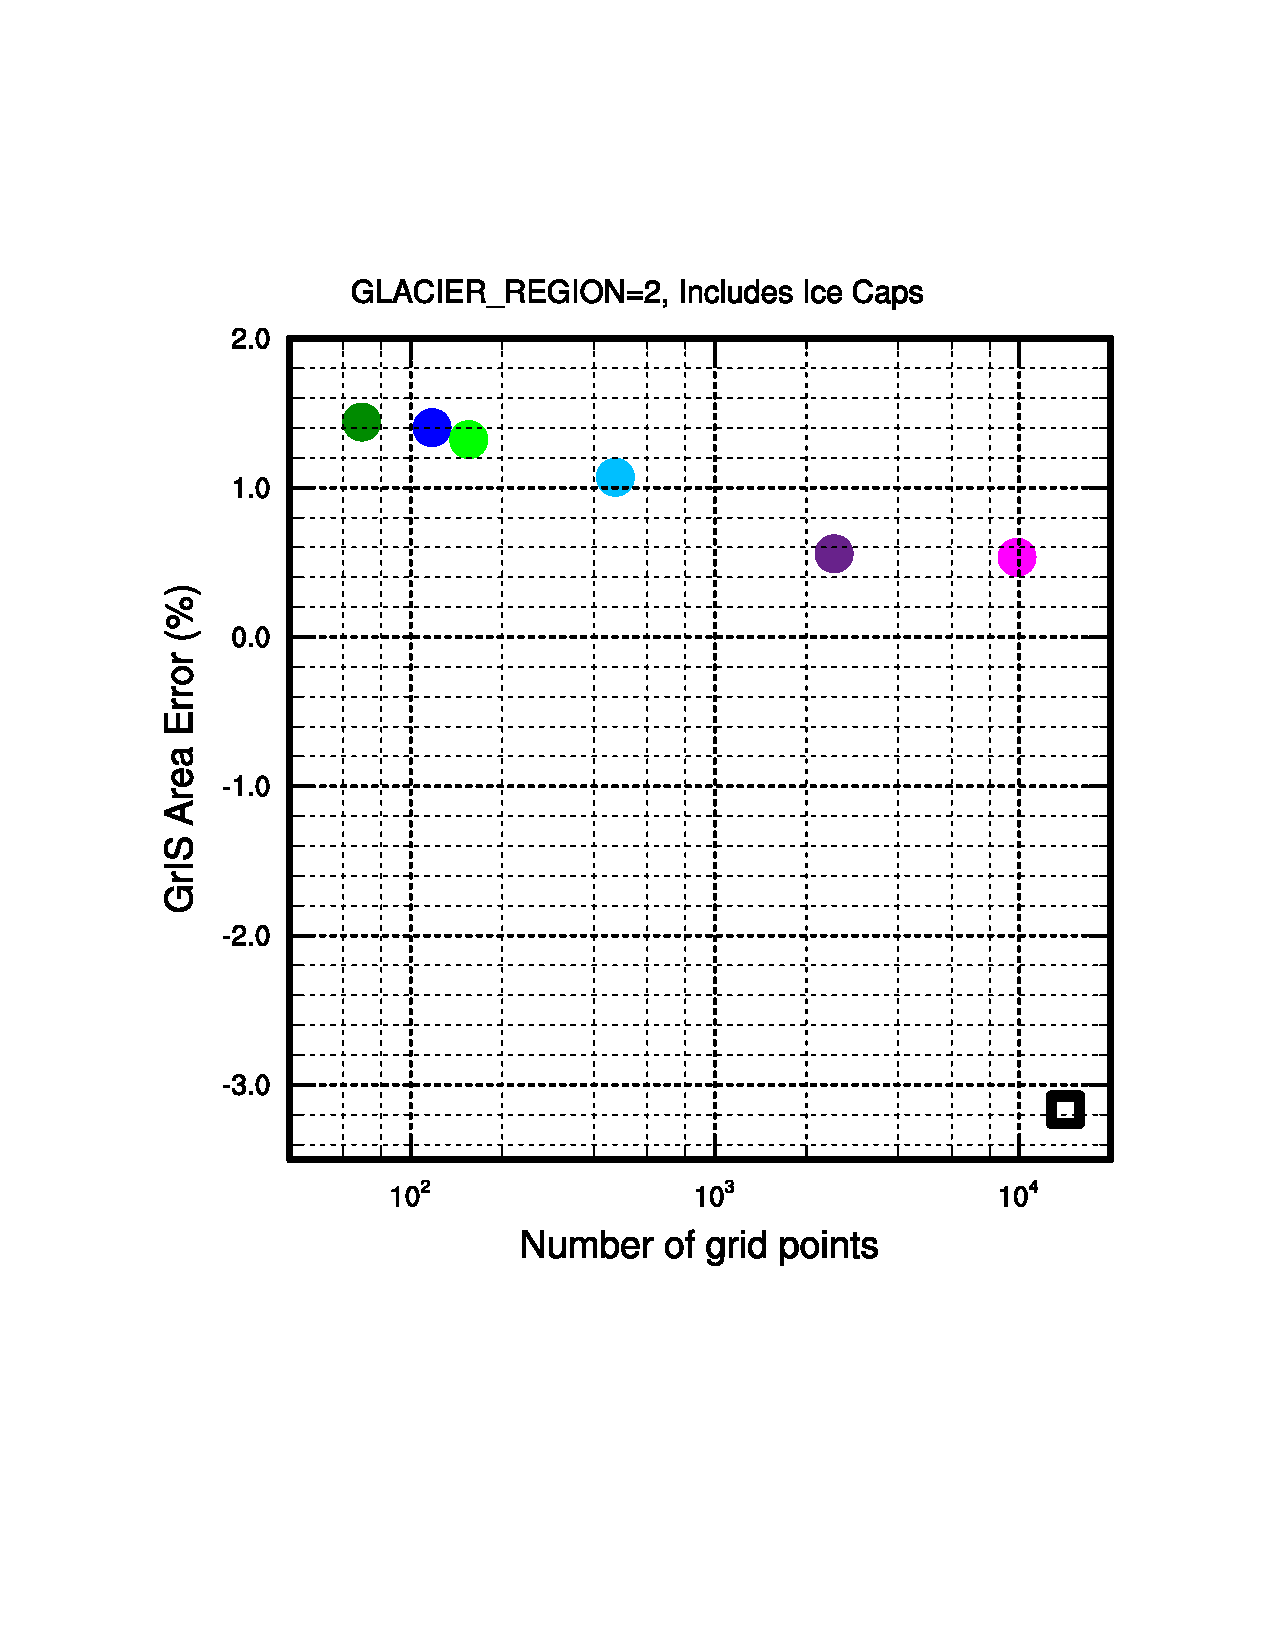
\includegraphics[width=60mm]{figs/temp_grisres_error.pdf} \\
\end{tabular}
\end{center}
\caption{.}
\label{fig:prect}
\end{figure}

\section{Methods}\label{sec:methods}
\subsection{Grids and dynamical cores}

The atmospheric component of CESM2.2, the Community Atmosphere Model, version 6.3 (CAM; \url{https://ncar.github.io/CAM/doc/build/html/index.html}), supports a diverse number of atmospheric dynamical cores. These range from dycores using latitude-longitude grids, the finite-volume \cite<FV;>{L2004MWR} and eulerian spectral transform \cite<EUL;>{CETAL006JC} models, and dycores built on unstructured grids, the spectral-element \cite<SE;>{LetAl2018JAMES} and finite-volume 3 \cite<FV3;>{PL2007JCP} models. The EUL dycore is the oldest dycore in CAM, and the least supported of all the dycores in the current model. FV3 is the newest dycore in CAM, but it was not fully incorporated at the time this work commenced, and so is omitted from this study. The authors instead focus on the two most well supported dycores in CAM, SE and FV.

\subsubsection{Finite-volume model}

The FV dycore is a hydrostatic model that integrates the equations of motion using a finite-volume discretization on a global latitude-longitude grid. The 2D dynamics evolve in floating Lagrangian layers that are periodically mapped to Eulerian reference grid in the vertical. Hyperviscous damping is applied to the divergent modes while Laplacian damping is applied to momentum in the top few layers, referred to as a ``sponge layer." A polar filter is used to avoid computational instability due to the convergence of the meridians, permitting the use of a more practical time-step. It takes the form of a Fourier filter in the zonal direction, with the damping coefficients increasing monotonically poleward.  The FV dycore is run with grids $\Delta x$ of $1^{\circ}$ and $2^{\circ}$ grid spacing, referred to as $f09$ and $f19$, respectively (Figure~\ref{fig:uni-grids}a,b).

\subsubsection{Spectral-element model}

The SE dycore is a hydrostatic model that integrates the equations of motion using a high-order continuous Galerkin method. The computational domain is defined by a cubed-sphere grid that is tiled with quasi-equal area quadralateral elements (e.g., Figure~\ref{fig:vr-grids}). Each element contains a fourth order basis set in the two horizontal directions, and the solution defined at the roots of the basis functions, the Gauss-Lobatto-Lagendre (GLL) quadrature points. This results in 16 GLL point values within each element, with 12 of the points lying on the element boundary. This compact support allows for efficient parallelization up to one element for task. Communication between elements happens via the direct stiffness summation, which applies a numerical flux to the element boundaries to reconcile overlapping nodal point values, and reulting in a continuous global basis set. 

As with the FV dycore, the dyanmics evolve in floating Lagrangian layers that are subsequently mapped to a Eulerian reference grid. The 2D dynamics have no implicit dissipation and so hyperviscosity operators are applied to all prognostic variables to remove spurious numerical errors. Laplacian damping is applied in the sponge layer, similar to the FV dycore.

The SE dycore supports regional grid refinement via its variable-resolution configuration. Two variable resolution meshes were developed as part of the CESM2.2 release that contains grid refinement over the Arctic. The software package SQuadgen (\url{https://github.com/ClimateGlobalChange/squadgen}) was used to generate these meshes. The $ARCTIC$ grid is a $\Delta x=1^{\circ}$ grid with $\Delta x=\frac{1}{4}^{\circ}$ regional refinement over the broader Arctic region. The $ARCTICGRIS$ grid is similar to the $ARCTIC$ grid, but additionally contains a patch covering the big island of Greenland with $\Delta x=\frac{1}{8}^{\circ}$ resolution. Both grids are depicted in Figure~\ref{fig:vr-grids}.

For spectral-element grids with quasi-uniform grid spacing, a variant in which tracer advection is computed using the Conservative Semi-Lagrangian Mulit-tracer tranport scheme is used instead \cite[CSLAM]{LTOUNGK2017MWR}. CSLAM has improved tracer property preservation and accelerated multi-tracer transport. It uses a seperate grid from the spectral-element dynamics, through dividing each element into $3\times3$ quasi-equal area control volumes. The physical parameterizations are computed from the state on the CSLAM grid, which has clear advantages over the default SE dycore in which the physics are evaluated at the GLL nodal points \cite{HL2018MWR}. 

The $1^{\circ}$ CAM-SE-CSLAM grid is referred to as $ne30pg3$ (Figure~\ref{fig:uni-grids}c). The $ne$ indicates the number of elements along an edge of a cubed-sphere face, and the $pg$ denotes the number of control volumes along the edge of an element used for computing the physical parameterizations. Optionally, one can compute the physics on a finite-volume grid that is $\frac{3}{2} \times \Delta x$ of the tracer-advection grid, found through dividing the elmenet into $2\times2$ control volumes \cite[(Figure~\ref{fig:uni-grids}d)]{HETAL2019JAMES}. A comparison of this lower-resolution physics grid $ne30pg2$ over the Arctic is included in this study. All variants of the SE dycore discussed herein are available as part of the CESM2.2 release.

\subsection{Physical parameterizations}

The CAM6 physical parameterization package (hereafter referred to as the \textit{physics}; \url{https://ncar.github.io/CAM/doc/build/html/index.html}) is used for all simulations in this study. CAM6 physics is most noteably different from it's predecessors through the incorporation of high-order turbulence closure, Cloud Layers Unified by Binormals \cite[CLUBB]{GETAL2002JAS,BOG2013JCLIM}, which jointly acts as a PBL, shallow convection and cloud macrophysics scheme. CLUBB is coupled with the MG2 microphysics scheme \cite{MG2}, with prognostic precipitation and classical nucleation theory in representing cloud ice for improved cloud-aerosol interactions. Deep convection is parameterized using a convective quasi-equilibrium mass flux scheme \cite{ZM1995AO,NRJ2008JC} inlcuding convective momentum transport \cite{RSG2010JAS}. PBL form drag is modeled after \cite{BBW2004QJRMS} and orographic gravity wave drag is represented with an anisotropic method driven by the orientation of topographic ridges at the sub-grid scale. 

\subsection{Experimental design}

All grids and dycores are run using an identical transient 1979-1998 AMIP-style configuration, with prescribed monthly SST/sea-ice after \cite{CESMSST}. This configuration refers to the $FHIST \ compset$ and runs out of the box in CESM2.2. The Community Land Model (CLM5; \url{https://escomp.github.io/ctsm-docs/versions/release-clm5.0/html/users_guide/index.html}) calculates the surface energy balance at each land tile within a grid cell, which is used to compute snow and bare ice melting to inform the surface mass balance (SMB) of a glacier unit \cite{VKETAL2020JGR}. Ice accumulation is modeled as a capping flux, or snow in excess of the assumed 10 m snow cap, and refreezing of liquid within the snowpack additionally acts as a source of mass in the SMB calculation. The SMB of the GrIS was spun-up for the variable-resolution grids by forcing CLM5 offline, cycling over 20 years of a fully coupled $ARCTIC$ run for about 500 years. The uniform resolution grids are all initialized with an SMB from an existing $f09$ spun-up initial condition. 

\subsection{Observational datasets}
\subsubsection{ERA5}
\subsubsection{LIVVkit 2.1}
\subsection{TempestExtremes}
\subsection{StormCompositer}

\section{Results}\label{sec:results}

\subsection{Tropospheric temperatures}
\subsection{Inter-annual variability}
\subsection{Synoptic-scale storm characteristics}
\subsection{Orographic gravity waves emanating from Greenland}
\subsection{Katabatic winds emanating from Greenland}
\subsection{Greenland surface mass balance}

% \section{Materials and Methods}
% Here is text on Materials and Methods.
%
% \subsection{A descriptive heading about methods}
% More about Methods.
%
% \section{Data} (Or section title might be a descriptive heading about data)
%
% \section{Results} (Or section title might be a descriptive heading about the
% results)
%

\section{Conclusions}\label{sec:conclusions}

\begin{figure}[t]
\begin{center}
         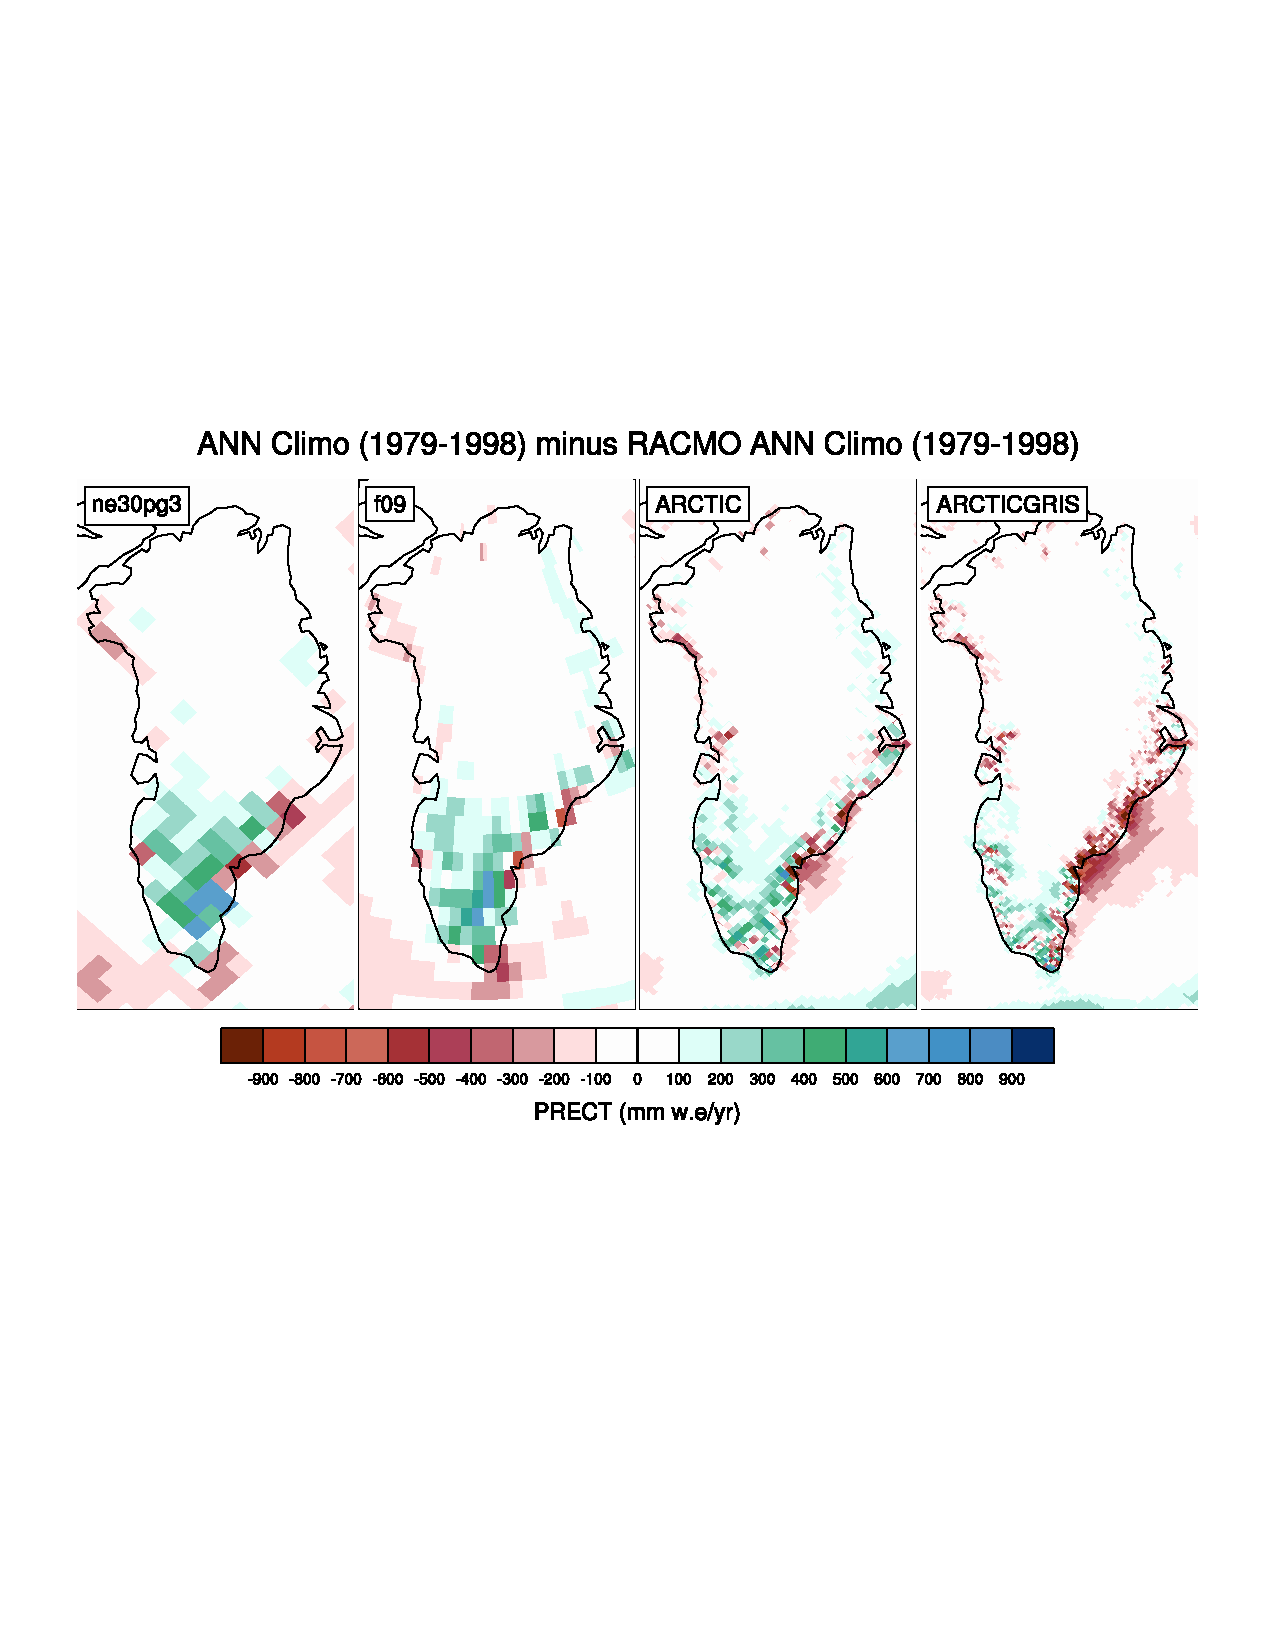
\includegraphics[width=130mm]{figs/temp_PRECT.pdf}
\end{center}
\caption{.}
\label{fig:prect}
\end{figure}

\begin{figure}[t]
\begin{center}
         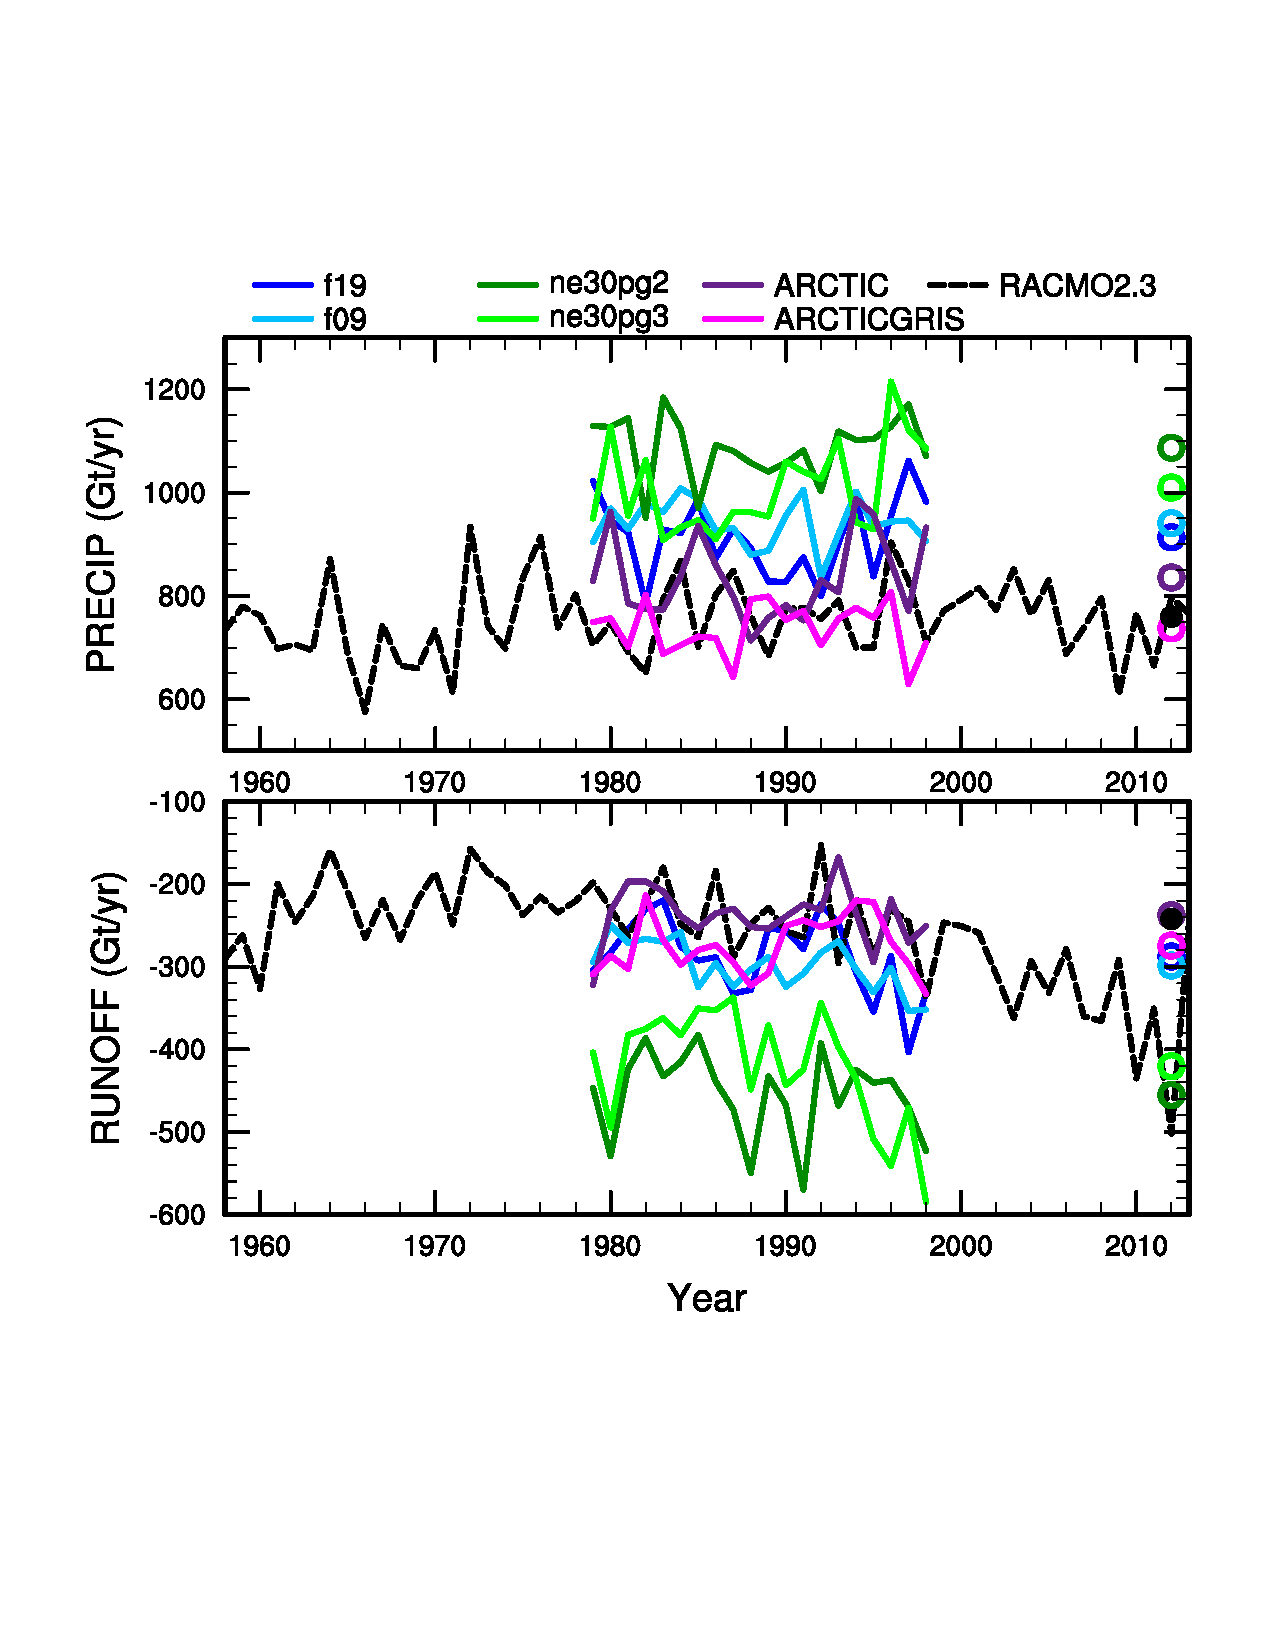
\includegraphics[width=100mm]{figs/temp_tseries_GRIS_map_TO_f19.pdf}
\end{center}
\caption{.}
\label{fig:tseries}
\end{figure}

\begin{figure}[t]
\begin{center}
         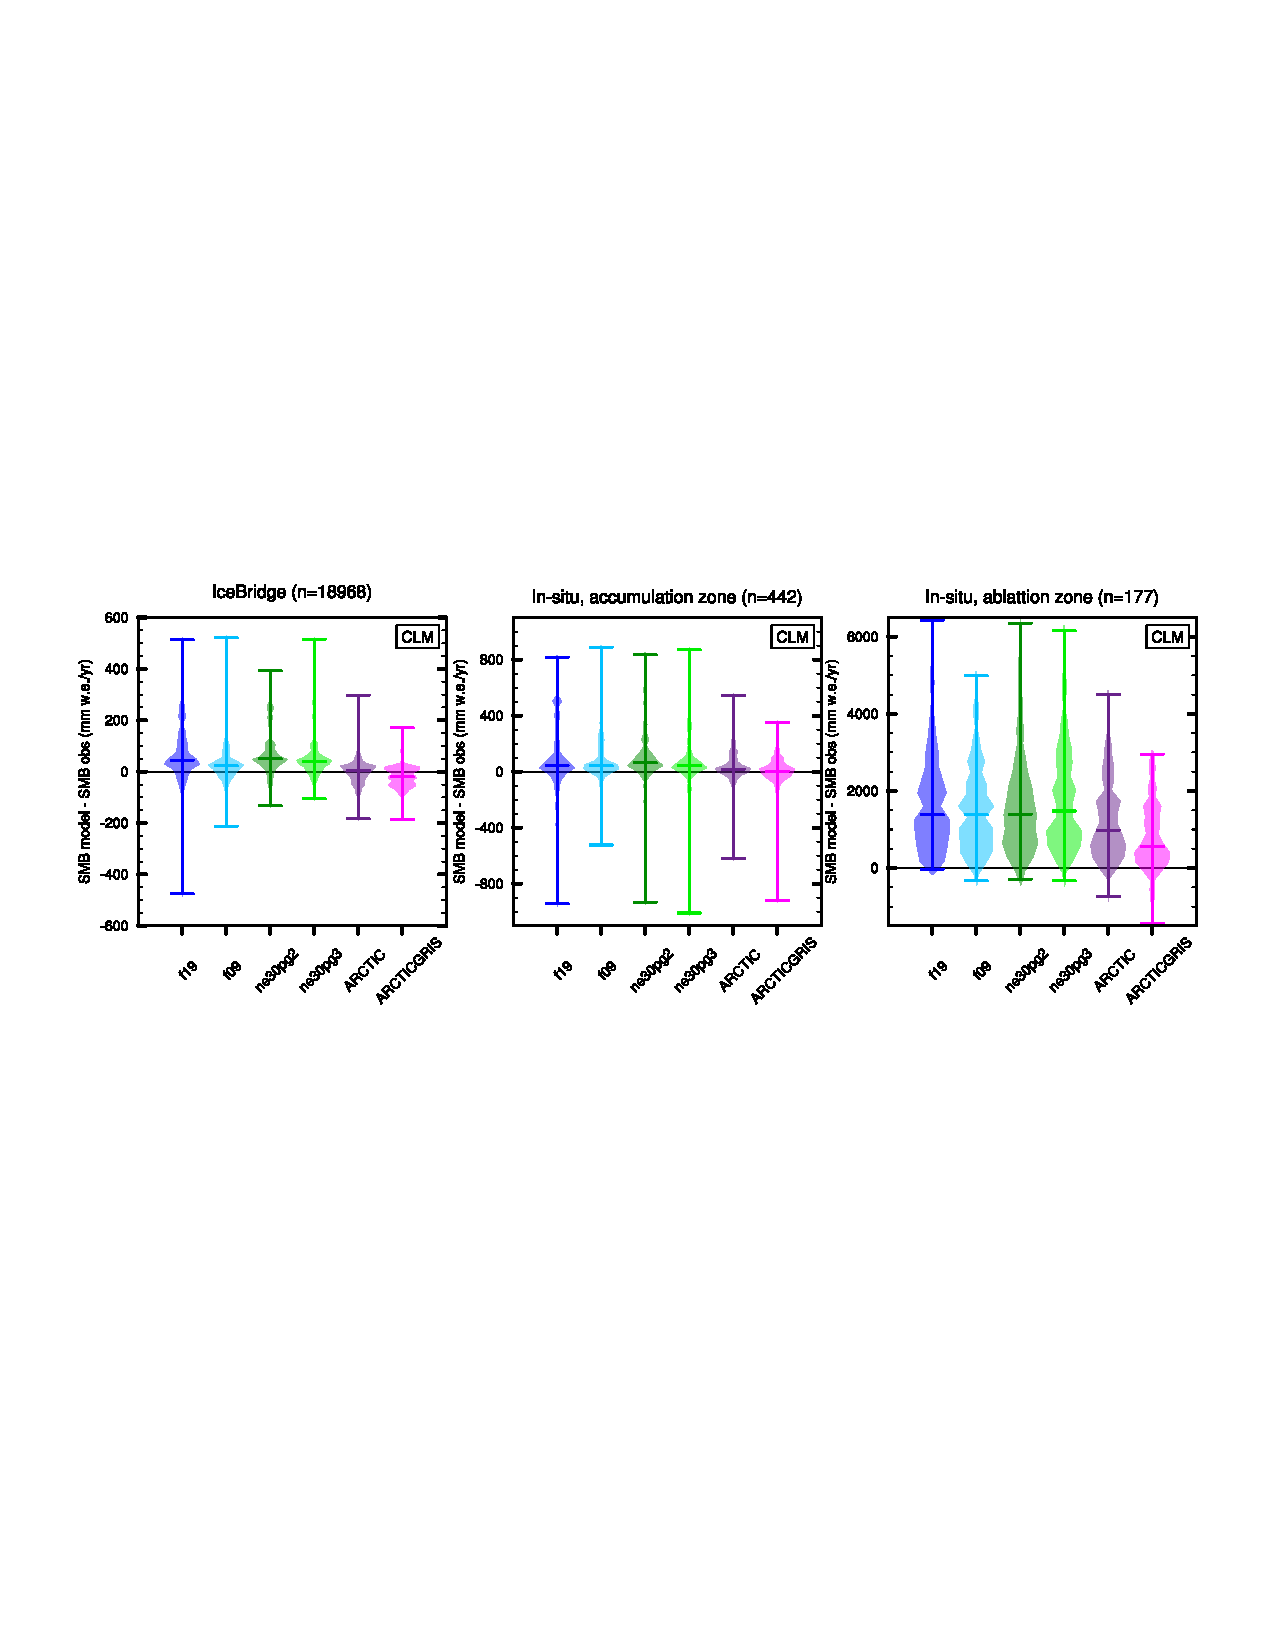
\includegraphics[width=130mm]{figs/temp_violens.pdf}
\end{center}
\caption{.}
\label{fig:pointdiff}
\end{figure}

\begin{figure}[t]
\begin{center}
\begin{tabular}{cccc}
         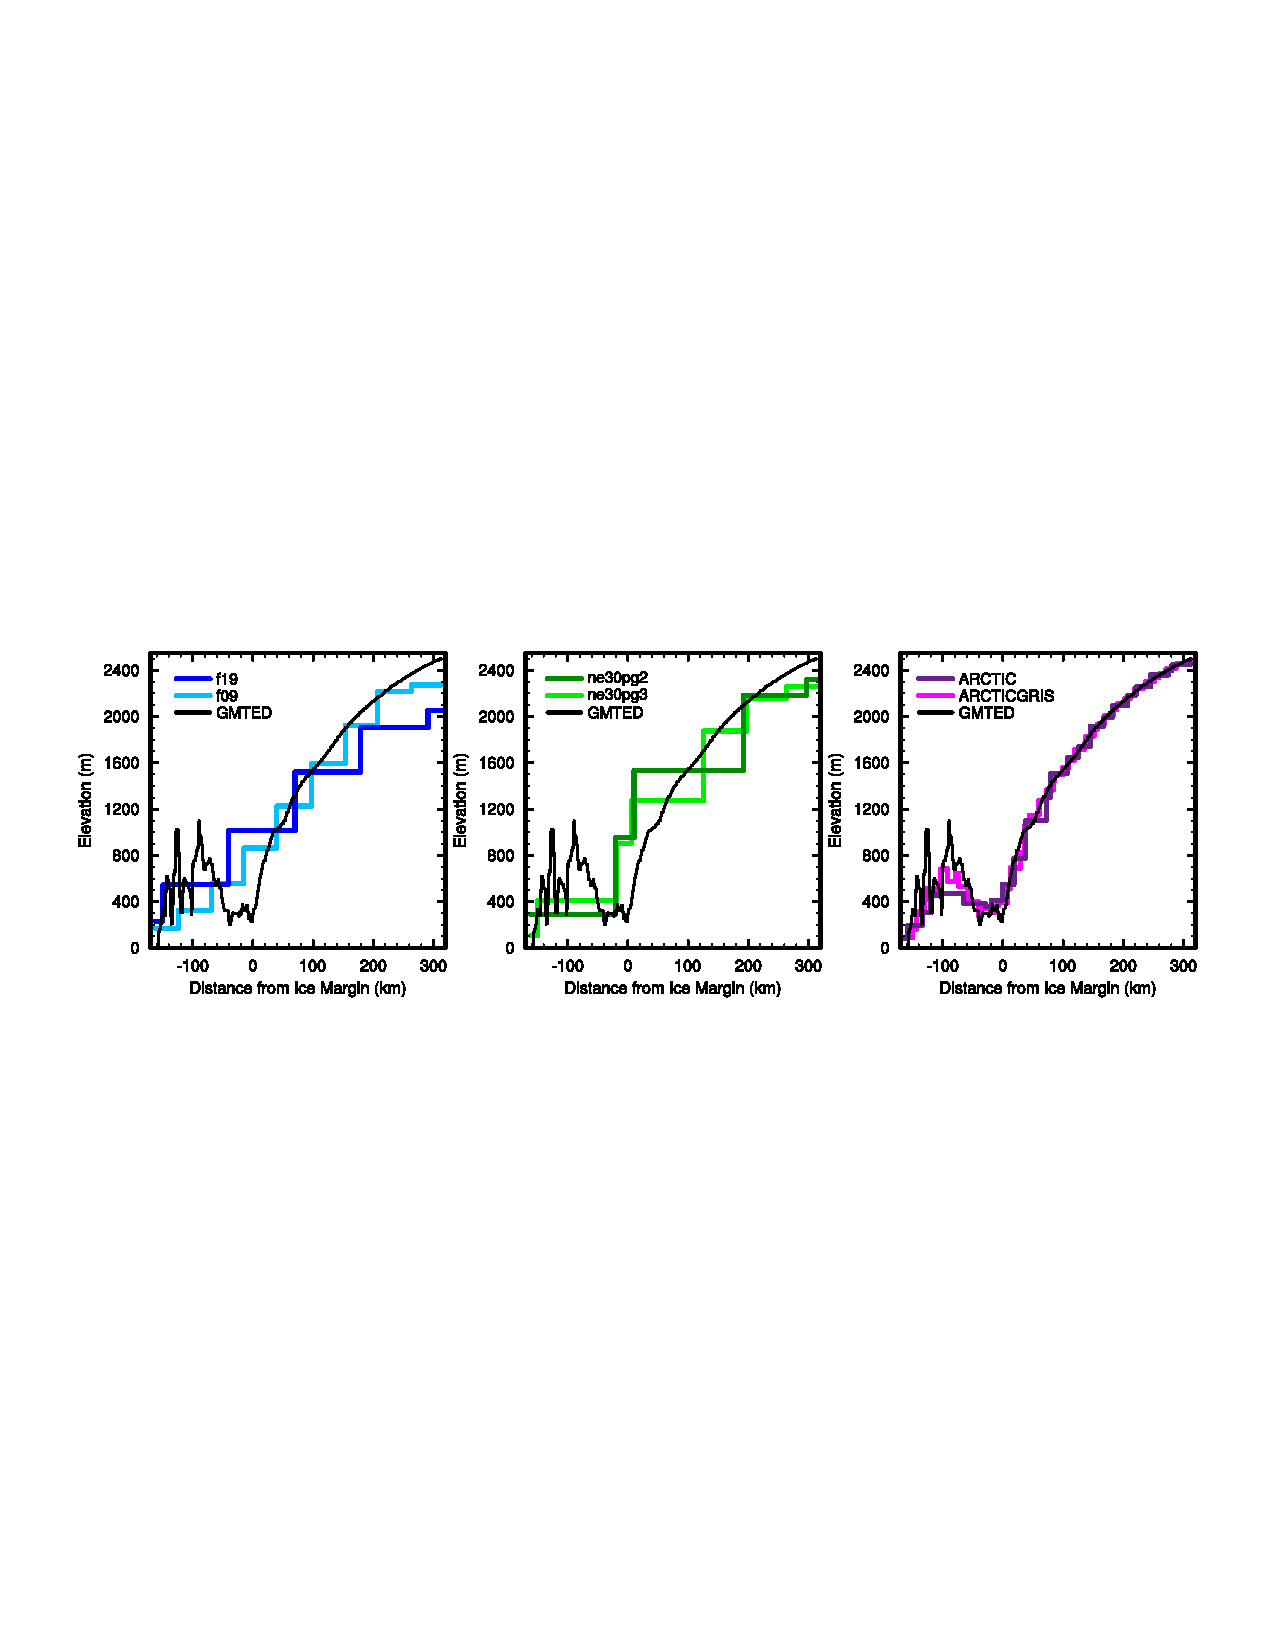
\includegraphics[width=100mm]{figs/temp_ktransect.pdf} \\
         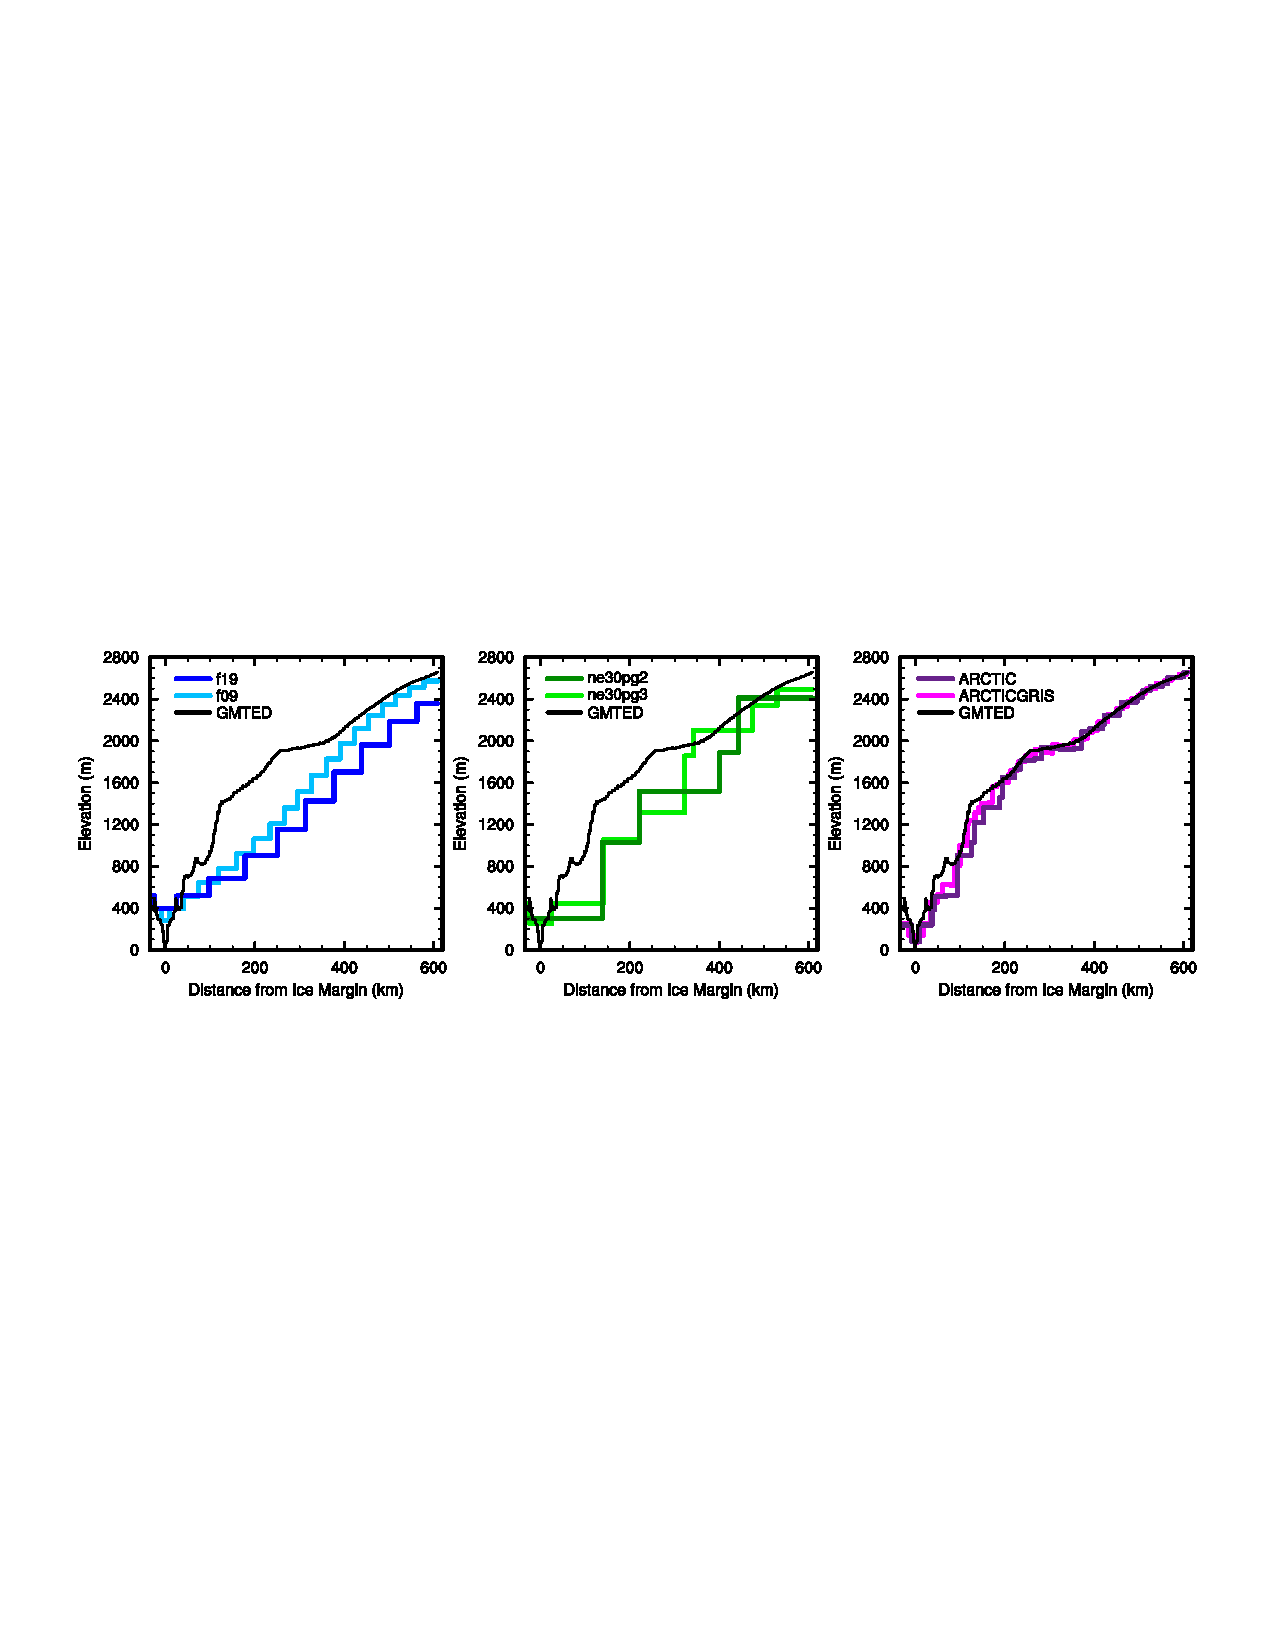
\includegraphics[width=100mm]{figs/temp_btransect.pdf} \\
\end{tabular}
\end{center}
\caption{.}
\label{fig:prect}
\end{figure}

\begin{figure}[t]
\begin{center}
\begin{tabular}{cccc}
         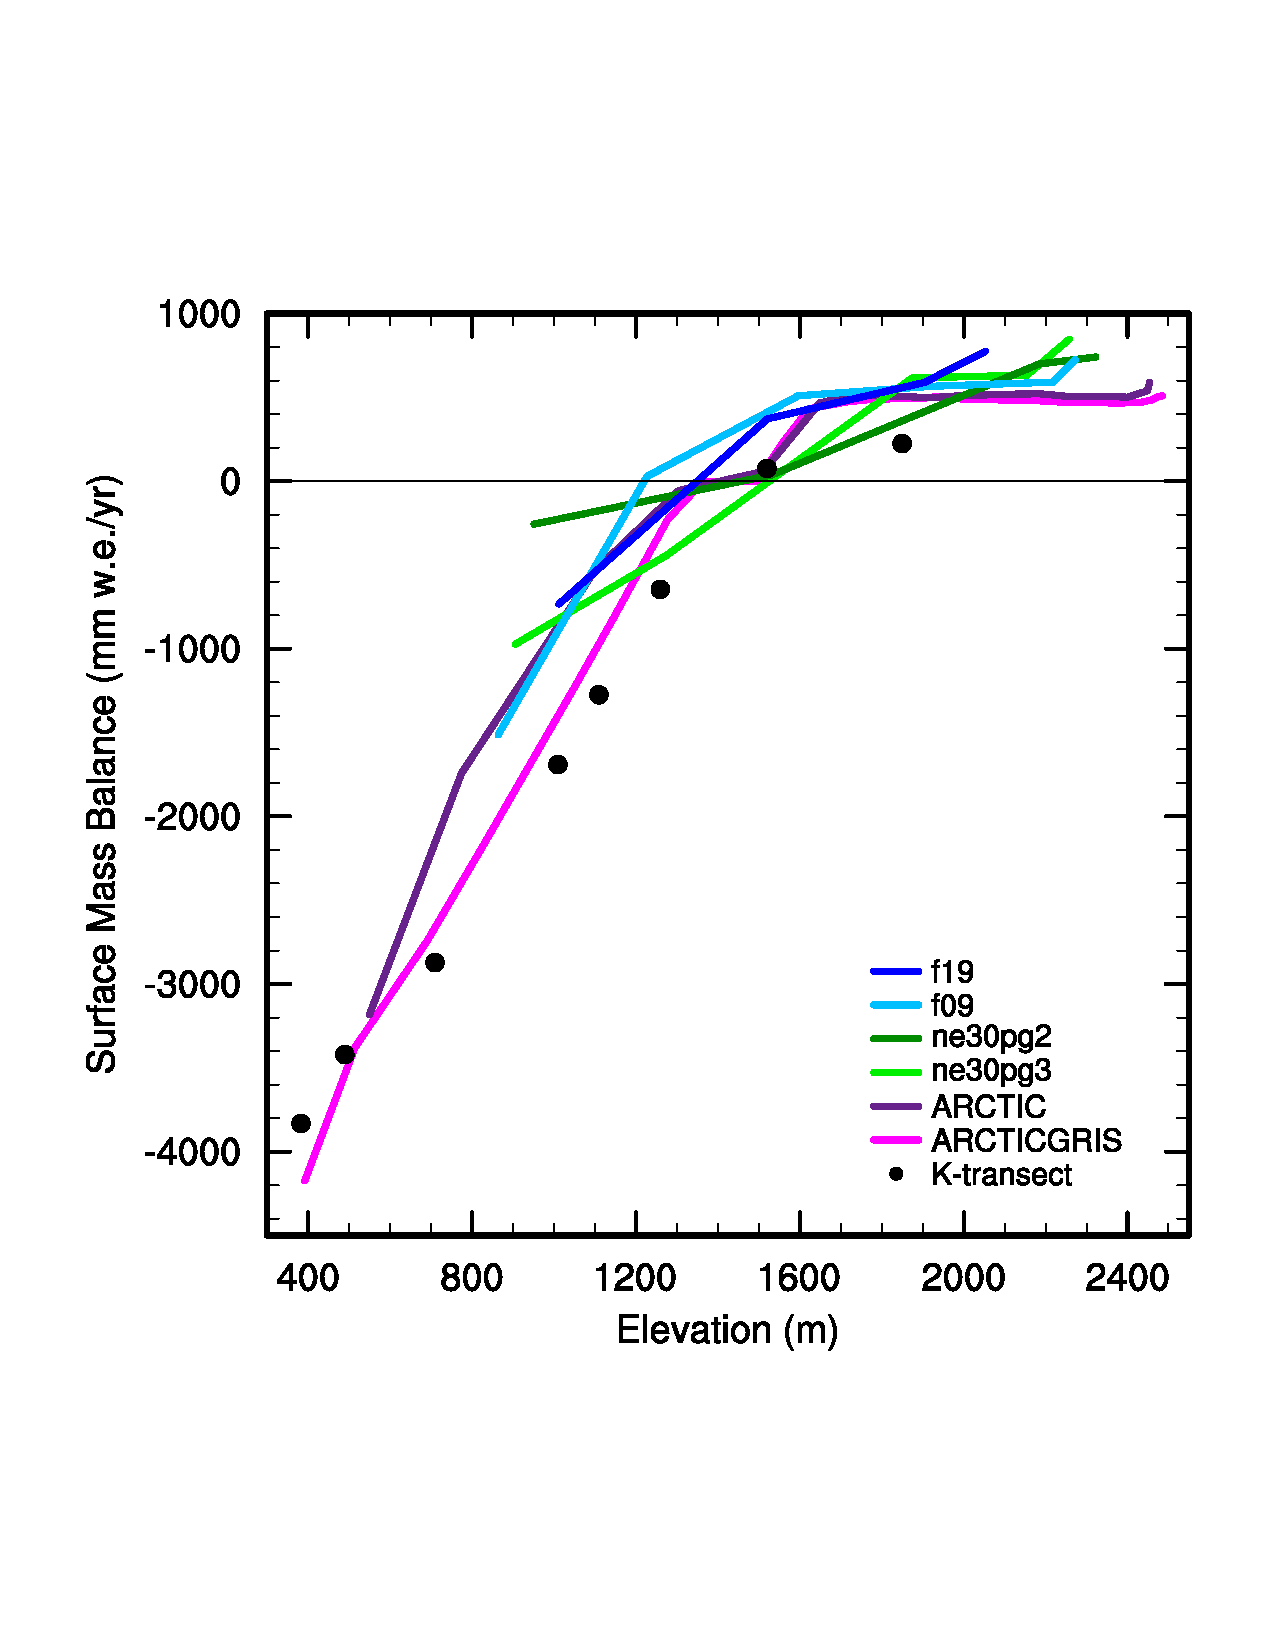
\includegraphics[width=60mm]{figs/temp_zsmb_ktrans_obsperiod.pdf}&
         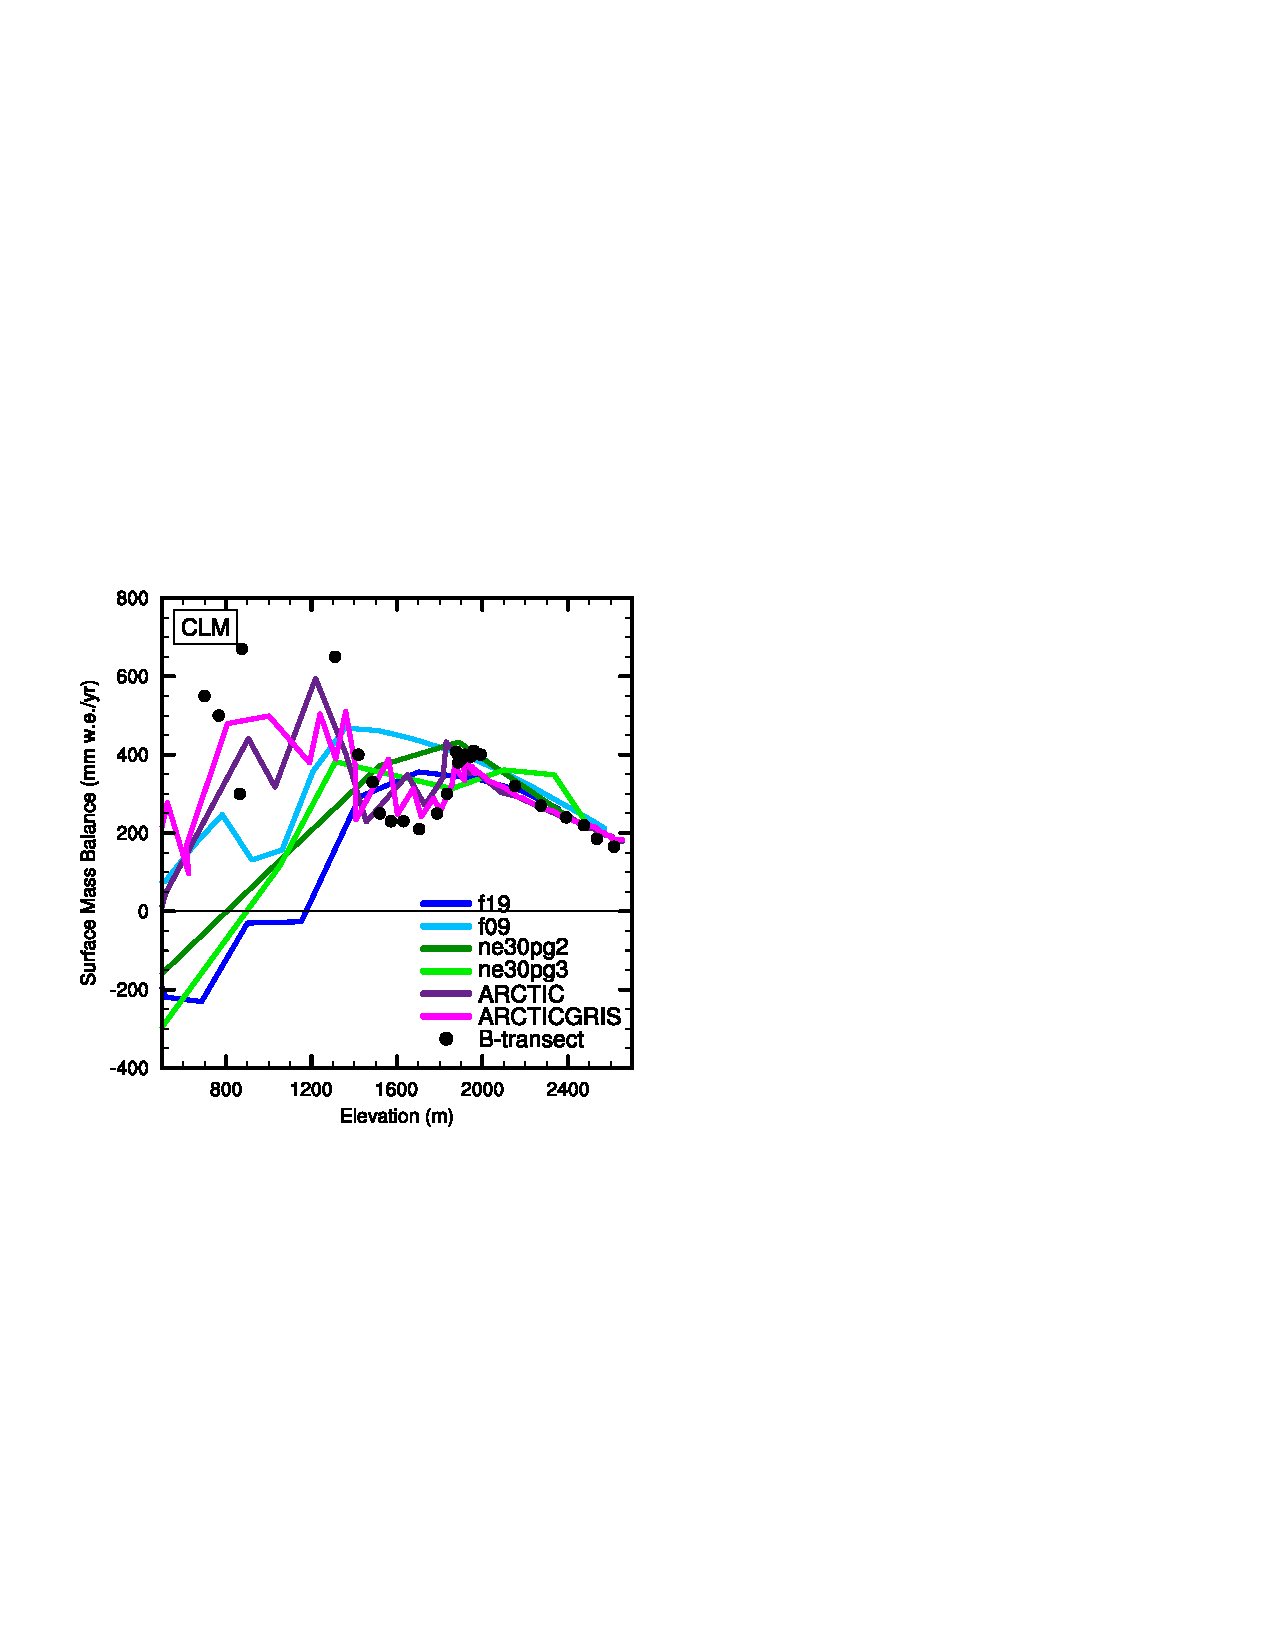
\includegraphics[width=60mm]{figs/temp_zsmb_btrans_obsperiod.pdf} \\
\end{tabular}
\end{center}
\caption{.}
\label{fig:prect}
\end{figure}

%Text here ===>>>


%%

%  Numbered lines in equations:
%  To add line numbers to lines in equations,
%  \begin{linenomath*}
%  \begin{equation}
%  \end{equation}
%  \end{linenomath*}



%% Enter Figures and Tables near as possible to where they are first mentioned:
%
% DO NOT USE \psfrag or \subfigure commands.
%
% Figure captions go below the figure.
% Table titles go above tables;  other caption information
%  should be placed in last line of the table, using
% \multicolumn2l{$^a$ This is a table note.}
%
%----------------
% EXAMPLE FIGURES
%
% \begin{figure}
% \includegraphics{example.png}
% \caption{caption}
% \end{figure}
%
% Giving latex a width will help it to scale the figure properly. A simple trick is to use \textwidth. Try this if large figures run off the side of the page.
% \begin{figure}
% \noindent\includegraphics[width=\textwidth]{anothersample.png}
%\caption{caption}
%\label{pngfiguresample}
%\end{figure}
%
%
% If you get an error about an unknown bounding box, try specifying the width and height of the figure with the natwidth and natheight options. This is common when trying to add a PDF figure without pdflatex.
% \begin{figure}
% \noindent\includegraphics[natwidth=800px,natheight=600px]{samplefigure.pdf}
%\caption{caption}
%\label{pdffiguresample}
%\end{figure}
%
%
% PDFLatex does not seem to be able to process EPS figures. You may want to try the epstopdf package.
%

%
% ---------------
% EXAMPLE TABLE
%
% \begin{table}
% \caption{Time of the Transition Between Phase 1 and Phase 2$^{a}$}
% \centering
% \begin{tabular}{l c}
% \hline
%  Run  & Time (min)  \\
% \hline
%   $l1$  & 260   \\
%   $l2$  & 300   \\
%   $l3$  & 340   \\
%   $h1$  & 270   \\
%   $h2$  & 250   \\
%   $h3$  & 380   \\
%   $r1$  & 370   \\
%   $r2$  & 390   \\
% \hline
% \multicolumn{2}{l}{$^{a}$Footnote text here.}
% \end{tabular}
% \end{table}

%% SIDEWAYS FIGURE and TABLE
% AGU prefers the use of {sidewaystable} over {landscapetable} as it causes fewer problems.
%
% \begin{sidewaysfigure}
% \includegraphics[width=20pc]{figsamp}
% \caption{caption here}
% \label{newfig}
% \end{sidewaysfigure}
%
%  \begin{sidewaystable}
%  \caption{Caption here}
% \label{tab:signif_gap_clos}
%  \begin{tabular}{ccc}
% one&two&three\\
% four&five&six
%  \end{tabular}
%  \end{sidewaystable}

%% If using numbered lines, please surround equations with \begin{linenomath*}...\end{linenomath*}
%\begin{linenomath*}
%\begin{equation}
%y|{f} \sim g(m, \sigma),
%\end{equation}
%\end{linenomath*}

%%% End of body of article

%%%%%%%%%%%%%%%%%%%%%%%%%%%%%%%%
%% Optional Appendix goes here
%
% The \appendix command resets counters and redefines section heads
%
% After typing \appendix
%
%\section{Here Is Appendix Title}
% will show
% A: Here Is Appendix Title
%
%\appendix
%\section{Here is a sample appendix}

%%%%%%%%%%%%%%%%%%%%%%%%%%%%%%%%%%%%%%%%%%%%%%%%%%%%%%%%%%%%%%%%
%
% Optional Glossary, Notation or Acronym section goes here:
%
%%%%%%%%%%%%%%
% Glossary is only allowed in Reviews of Geophysics
%  \begin{glossary}
%  \term{Term}
%   Term Definition here
%  \term{Term}
%   Term Definition here
%  \term{Term}
%   Term Definition here
%  \end{glossary}

%
%%%%%%%%%%%%%%
% Acronyms
%   \begin{acronyms}
%   \acro{Acronym}
%   Definition here
%   \acro{EMOS}
%   Ensemble model output statistics
%   \acro{ECMWF}
%   Centre for Medium-Range Weather Forecasts
%   \end{acronyms}

%
%%%%%%%%%%%%%%
% Notation
%   \begin{notation}
%   \notation{$a+b$} Notation Definition here
%   \notation{$e=mc^2$}
%   Equation in German-born physicist Albert Einstein's theory of special
%  relativity that showed that the increased relativistic mass ($m$) of a
%  body comes from the energy of motion of the body—that is, its kinetic
%  energy ($E$)—divided by the speed of light squared ($c^2$).
%   \end{notation}




%%%%%%%%%%%%%%%%%%%%%%%%%%%%%%%%%%%%%%%%%%%%%%%%%%%%%%%%%%%%%%%%
%
%  ACKNOWLEDGMENTS
%
% The acknowledgments must list:
%
% >>>>	A statement that indicates to the reader where the data
% 	supporting the conclusions can be obtained (for example, in the
% 	references, tables, supporting information, and other databases).
%
% 	All funding sources related to this work from all authors
%
% 	Any real or perceived financial conflicts of interests for any
%	author
%
% 	Other affiliations for any author that may be perceived as
% 	having a conflict of interest with respect to the results of this
% 	paper.
%
%
% It is also the appropriate place to thank colleagues and other contributors.
% AGU does not normally allow dedications.


\acknowledgments
This material is based upon work supported by the National Center for Atmospheric Research (NCAR), which is a major facility sponsored by the NSF under Cooperative Agreement 1852977. Computing and data storage resources, including the Cheyenne supercomputer
(doi:10.5065/D6RX99HX), were provided by the Computational and Information Systems Laboratory (CISL) at NCAR.

The data presented in this manuscript is available at {\url{https://github.com/adamrher/2020-arcticgrids}}.



%% ------------------------------------------------------------------------ %%
%% References and Citations

%%%%%%%%%%%%%%%%%%%%%%%%%%%%%%%%%%%%%%%%%%%%%%%
%
% \bibliography{<name of your .bib file>} don't specify the file extension
%
% don't specify bibliographystyle
%%%%%%%%%%%%%%%%%%%%%%%%%%%%%%%%%%%%%%%%%%%%%%%

%\bibliography{ enter your bibtex bibliography filename here }
\bibliography{bib}


%Reference citation instructions and examples:
%
% Please use ONLY \cite and \citeA for reference citations.
% \cite for parenthetical references
% ...as shown in recent studies (Simpson et al., 2019)
% \citeA for in-text citations
% ...Simpson et al. (2019) have shown...
%
%
%...as shown by \citeA{jskilby}.
%...as shown by \citeA{lewin76}, \citeA{carson86}, \citeA{bartoldy02}, and \citeA{rinaldi03}.
%...has been shown \cite{jskilbye}.
%...has been shown \cite{lewin76,carson86,bartoldy02,rinaldi03}.
%... \cite <i.e.>[]{lewin76,carson86,bartoldy02,rinaldi03}.
%...has been shown by \cite <e.g.,>[and others]{lewin76}.
%
% apacite uses < > for prenotes and [ ] for postnotes
% DO NOT use other cite commands (e.g., \citet, \citep, \citeyear, \nocite, \citealp, etc.).
%



\end{document}



More Information and Advice:

%% ------------------------------------------------------------------------ %%
%
%  SECTION HEADS
%
%% ------------------------------------------------------------------------ %%

% Capitalize the first letter of each word (except for
% prepositions, conjunctions, and articles that are
% three or fewer letters).

% AGU follows standard outline style; therefore, there cannot be a section 1 without
% a section 2, or a section 2.3.1 without a section 2.3.2.
% Please make sure your section numbers are balanced.
% ---------------
% Level 1 head
%
% Use the \section{} command to identify level 1 heads;
% type the appropriate head wording between the curly
% brackets, as shown below.
%
%An example:
%\section{Level 1 Head: Introduction}
%
% ---------------
% Level 2 head
%
% Use the \subsection{} command to identify level 2 heads.
%An example:
%\subsection{Level 2 Head}
%
% ---------------
% Level 3 head
%
% Use the \subsubsection{} command to identify level 3 heads
%An example:
%\subsubsection{Level 3 Head}
%
%---------------
% Level 4 head
%
% Use the \subsubsubsection{} command to identify level 3 heads
% An example:
%\subsubsubsection{Level 4 Head} An example.
%
%% ------------------------------------------------------------------------ %%
%
%  IN-TEXT LISTS
%
%% ------------------------------------------------------------------------ %%
%
% Do not use bulleted lists; enumerated lists are okay.
% \begin{enumerate}
% \item
% \item
% \item
% \end{enumerate}
%
%% ------------------------------------------------------------------------ %%
%
%  EQUATIONS
%
%% ------------------------------------------------------------------------ %%

% Single-line equations are centered.
% Equation arrays will appear left-aligned.

Math coded inside display math mode \[ ...\]
 will not be numbered, e.g.,:
 \[ x^2=y^2 + z^2\]

 Math coded inside \begin{equation} and \end{equation} will
 be automatically numbered, e.g.,:
 \begin{equation}
 x^2=y^2 + z^2
 \end{equation}


% To create multiline equations, use the
% \begin{eqnarray} and \end{eqnarray} environment
% as demonstrated below.
\begin{eqnarray}
  x_{1} & = & (x - x_{0}) \cos \Theta \nonumber \\
        && + (y - y_{0}) \sin \Theta  \nonumber \\
  y_{1} & = & -(x - x_{0}) \sin \Theta \nonumber \\
        && + (y - y_{0}) \cos \Theta.
\end{eqnarray}

%If you don't want an equation number, use the star form:
%\begin{eqnarray*}...\end{eqnarray*}

% Break each line at a sign of operation
% (+, -, etc.) if possible, with the sign of operation
% on the new line.

% Indent second and subsequent lines to align with
% the first character following the equal sign on the
% first line.

% Use an \hspace{} command to insert horizontal space
% into your equation if necessary. Place an appropriate
% unit of measure between the curly braces, e.g.
% \hspace{1in}; you may have to experiment to achieve
% the correct amount of space.


%% ------------------------------------------------------------------------ %%
%
%  EQUATION NUMBERING: COUNTER
%
%% ------------------------------------------------------------------------ %%

% You may change equation numbering by resetting
% the equation counter or by explicitly numbering
% an equation.

% To explicitly number an equation, type \eqnum{}
% (with the desired number between the brackets)
% after the \begin{equation} or \begin{eqnarray}
% command.  The \eqnum{} command will affect only
% the equation it appears with; LaTeX will number
% any equations appearing later in the manuscript
% according to the equation counter.
%

% If you have a multiline equation that needs only
% one equation number, use a \nonumber command in
% front of the double backslashes (\\) as shown in
% the multiline equation above.

% If you are using line numbers, remember to surround
% equations with \begin{linenomath*}...\end{linenomath*}

%  To add line numbers to lines in equations:
%  \begin{linenomath*}
%  \begin{equation}
%  \end{equation}
%  \end{linenomath*}



